\documentclass[fr]{../../../eplsummary}

\usepackage{dafny}
\usepackage{../../../eplcode}
\usepackage{float}
\usepackage{multicol}
\usepackage{booktabs}

\newcommand{\seqcomp}{\,{;}\,}
\newcommand{\dtree}{D_{\texttt{Tree}}}
\newcommand{\prectree}{\prec_{\texttt{Tree}}}
\newcommand{\letree}{<_{\texttt{Tree}}}

\DeclareMathOperator{\absf}{abs}
\DeclareMathOperator{\ok}{ok}
\DeclareMathOperator{\weakest}{wp}

\lstset{language=dafny}

\hypertitle{Méthodes de conception de programmes}{6}{INGI}{1122}
{Gilles Peiffer\and Liliya Semerikova}
{Charles Pecheur}

\section{Introduction}
\subsection{Une science de la programmation}
\subsubsection{Programmes et bugs}
\begin{mydef}
	Le \emph{débogage} consiste à programmer,
	tester et corriger le programme jusqu'à ne plus trouver d'erreurs.
	C'est inefficace en tant que méthodologie
	car c'est incertain pour établir la correction et trouver les erreurs.
	Pour ça on utilisera plutôt la science de la programmation:
	\begin{itemize}
		\item \emph{spécifier} les programmes;
		\item \emph{vérifier} les programmes
		par rapport à leurs spécifications;
		\item \emph{construire} les programmes
		sur base de leurs spécifications;
	\end{itemize}
\end{mydef}

\subsection{Problème, solution et preuve}
\subsubsection{Théorie du problème}
Pour définir la théorie du problème,
on réfléchit d'abord aux \emph{structures},
aux \emph{opérations} et \emph{caractéristiques} qui interviennent
et à leurs \emph{propriétés} utiles.
Ensuite, on résout le problème et on vérifie
si la solution trouvée est correcte
par rapport aux spécifications du problème (pré-/postconditions).
Pour finir, on représente la solution sous forme de programme.

\subsubsection{Correction}
\begin{mydef}
	Les concepts suivants permettent de formaliser
	la notion d'un programme correct.
	\begin{itemize}
		\item \emph{Correction}:
		si les données satisfont les préconditions,
		alors les résultats satisfont les postconditions.
		\item \emph{Terminaison}:
		si les données satisfont les préconditions,
		alors le programme se termine.
		\item \emph{Correction partielle}:
		si les données satisfont les préconditions
		et si le programme se termine,
		alors les résultats satisfont les postconditions.
		\item \emph{Correction totale}:
		si les données satisfont les préconditions,
		alors le programme se termine
		et les résultats satisfont les postconditions.
		On a donc que la correction totale est équivalente
		à la correction partielle à laquelle on ajoute la terminaison.
	\end{itemize}
\end{mydef}

\subsubsection{Preuve}
On prouve la terminaison grâce au \emph{variant}
qui est un \emph{nombre fini positif ou nul} et qui,
pour un programme qui se termine, \emph{dimininue} à chaque itération.
Le \emph{nombre d'itérations est aussi fini}.
On prouve la correction partielle en trouvant un \emph{invariant de boucle},
c'est-à-dire un prédicat satisfait tout au long de l'exécution du programme.
Pour cette preuve, on établit que
\begin{itemize}
	\item Si les \emph{préconditions} sont vraies \emph{initialement},
	alors l'\emph{invariant} est vrai à l'entrée dans la boucle.
	\item Si l'\emph{invariant} est vrai
	avant une \emph{itération de la boucle},
	alors l'\emph{invariant} est vrai après l'itération.
	\item Si l'\emph{invariant} est vrai à la sortie de la boucle
	alors les \emph{postconditions} sont vraies \emph{finalement}.
\end{itemize}

La preuve sur l'itération est une preuve par récurrence.
Il y a un cas de base pour montrer que
l'invariant est vrai après zéro itérations.
Ensuite, on a un cas inductif où on prouve que,
si l'invariant est vrai après $N$ itérations,
alors il l'est aussi après $N+1$ itérations.
On conclut donc que l'invariant est toujours vrai.

\subsubsection{Précision}
Afin de pouvoir prouver ceci,
il faut \emph{définir} de façon \emph{précise} et \emph{non ambigüe}
\begin{itemize}
	\item la \emph{spécification},
	qui dit \emph{ce que le programme doit calculer}
	en utilisant un \emph{langage de spécification},
	\item le \emph{programme},
	qui dit \emph{comment} le programme doit calculer
	en utilisant un \emph{langage de programmation}
	(instructions exécutables),
	\item la \emph{preuve},
	qui \emph{justifie} que le programme \emph{satisfait} la spécification
	en utilisant des \emph{règles de preuve}.
\end{itemize}

\subsubsection{Représentation}
Pour implémenter cela \emph{dans un programme},
on recherche une \emph{représentation} pour les \emph{données}
(structures, opérations, attributs),
pour le \emph{problème} (spécification),
pour la \emph{solution} (programme)
et pour la preuve (variants, invariants).

\section{Programmes simples}
\subsection{Spécification de programmes}
\subsubsection{Assertions de programme}

\begin{mydef}
	Une \emph{assertion} est une formule en logique des prédicats
	vraie en un point du programme.
	On la note $[p]$, où $p$ comporte des variables du programme
	et est vraie.
\end{mydef}

\subsubsection{Triplet de Hoare}
\begin{mydef}
	Un \emph{triplet de Hoare} est noté $[P]\ S\ [Q]$,
	où les prédicats $P$ et $Q$ sont la pré- et postcondition
	et $S$ est le programme.
	Un tel triplet est une proposition logique
	qui peut être \emph{valide} ou \emph{invalide}.

	Le triplet $[P]\ S\ [Q]$ est \emph{valide} si et seulement si:
	Si $P$ est \emph{vrai avant} d'exécuter $S$,
	alors l'éxecution de $S$ \emph{se termine}
	et $Q$
	est \emph{vraie après}
	l'éxecution de $S$.\footnote{Cela implique
	que si le prédicat $P$ est faux, alors le triplet est d'office valide.}
	C'est une condition de \emph{correction totale};
	on dit que $S$ \emph{réalise} $Q$
	sous l'\emph{assomption} de $P$.
\end{mydef}
On dira par ailleurs que le résultat d'un programme
est toujours stocké dans la variable $r$.

\subsubsection{Variables auxiliaires}
\begin{mydef}
	Les \emph{variables auxiliaires} ne sont \emph{pas}
	des variables du programme.
	Leur valeur \emph{ne change pas} au cours de l'exécution:
	elles sont \emph{rigides}.
\end{mydef}
Les variables auxiliaires se notent soit avec une lettre majuscule,
soit avec un indice \og ${}_0$ \fg, soit avec les deux.

\subsubsection{Tableau d'assertions}
Grâce aux triplets de Hoare, on peut examiner
chaque ligne d'un programme à son tour,
en spécifiant les préconditions et les postconditions pour chaque,
de sorte à ce que la postcondition pour la ligne $i$
soit la précondition pour la ligne $i+1$.
On parle d'un \emph{tableau d'assertions}.

\subsubsection{Conséquence}
\begin{mydef}
	La \emph{conséquence} est un \emph{connecteur logique}
	qui peut modifier des pré- ou postconditions.
	Il est toujours possible dans un triplet de Hoare
	de remplacer un prédicat par une conséquence de celui-ci.
	\begin{itemize}
		\item Dans le cas de la précondition,
		elle crée un \emph{renforcement} de la \emph{précondition}.
		On remplace la précondition actuelle
		par une précondition \emph{plus contraignante}
		dont la précondition initiale se déduit.
		\item Dans le cas de la postcondition,
		elle crée un \emph{affaiblissement} de la \emph{postcondition}.
		On remplace la postcondition actuelle
		par une postcondition \emph{moins contraignante}
		qui se déduit de la postcondition initiale.
	\end{itemize}

	La règle de conséquence est donc
	\og si $P \implies Q$, alors $[P][Q]$ \fg.
\end{mydef}

\subsection{Affectation}
\begin{mydef}
	Une \emph{affectation} est une structure de la forme $V \coloneqq E$,
	où $V$ est une \emph{variable} et $E$ est une \emph{expression}.
	Il est possible de faire une \emph{affectation simultanée},
	de la forme $V_1, \ldots, V_n \coloneqq E_1, \ldots, E_n$.
	La partie de gauche est une liste de variables
	et la partie de droite est une liste d'expressions, de la même taille.
\end{mydef}

\begin{mynota}
	On définit la notation $Q[V \coloneqq E]$,
	qui signifie \og $Q$ où toutes les occurrences de $V$
	sont remplacées par $E$\fg.
\end{mynota}
On définit alors l'\emph{axiome d'affectation} suivant:
\begin{equation}
	[Q[V \coloneqq E]]\ V \coloneqq E\ [Q]\,.
\end{equation}
On le fait en arrière où à partir de $Q$ on va calculer $Q[V\coloneqq E]$.
De façon similaire, \emph{l'axiome de l'affectation simultanée} se note
\begin{equation}
	[Q[V_1, \ldots, V_n \coloneqq E_1, \ldots, E_n]]\ V_1, \ldots, V_n \coloneqq E_1, \ldots, E_n\ [Q]\,.
\end{equation}

Il existe un forme alternative pour les axiomes de l'affectation:
\begin{align}
	[Q[E]]\ V &\coloneqq E\ [Q[V]]\,,\\
	[Q[E_1, \ldots, E_n]]\ V_1, \ldots, V_n &\coloneqq E_1, \ldots, E_n\ [Q[V_1, \ldots, V_n]]\,.
\end{align}
en sachant que $Q[V] = Q$ où $V$ apparaît
et $Q[E] = Q[V]$ où $V$ est remplacé par $E$.

\begin{figure}[H]
	\centering
	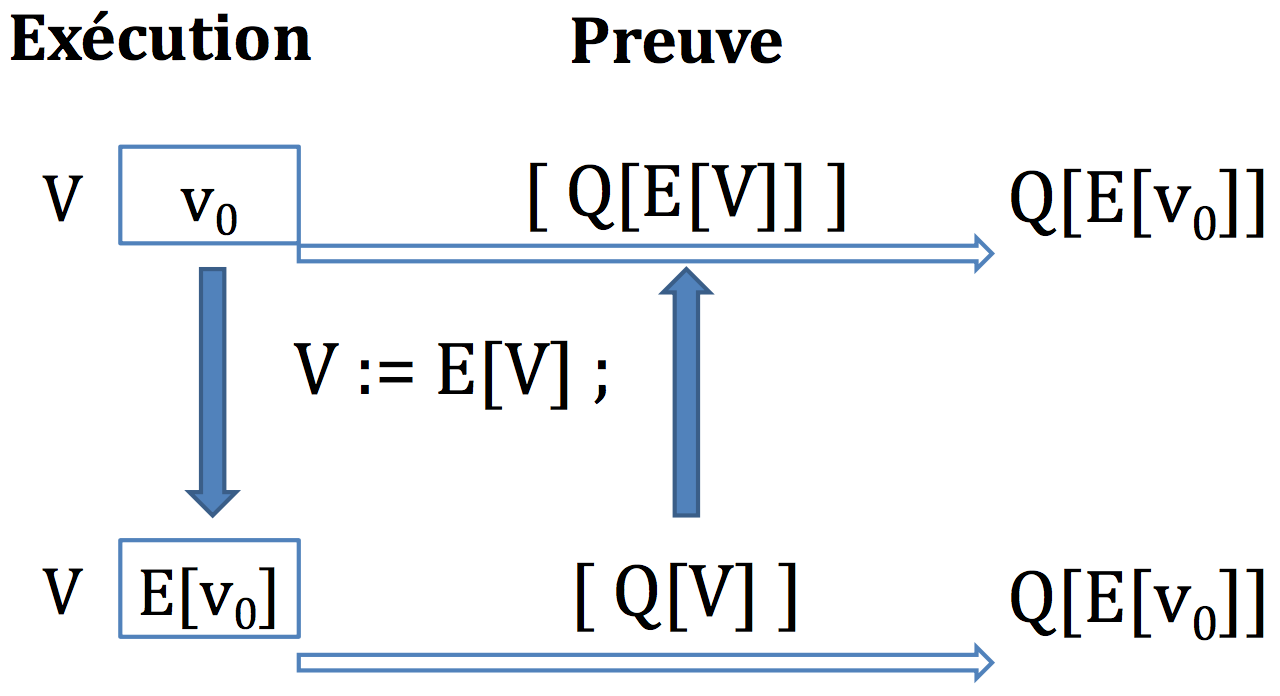
\includegraphics[width=0.7\textwidth]{img/assignment}
	\caption{Affectation: exécution et preuve.}
\end{figure}

\subsection{Séquences}
Une des stratégies utilisées pour résoudre un problème
est de le décomposer en deux (ou plus) sous-problèmes faciles
et de les résoudre dans un ordre spécifique.
En langage informatique,
on résout ce problème par la \emph{composition séquentielle}.
\begin{mynota}
	La composition séquentielle de $S1$ et $S2$ se note $S1 \seqcomp S2$.
\end{mynota}
La composition séquentielle est \emph{associative}:
$(S1 \seqcomp S2) \seqcomp S3 = S1 \seqcomp (S1 \seqcomp S3) = S1 \seqcomp S2 \seqcomp S3$.
Supposons un programme spécifié par la précondition $P$
et par la postcondition $Q$.
On veut écrire une instruction $S$ pour satisfaire $[P]\ S\ [Q]$.
Pour cela, on décompose le problème en deux sous-problèmes $S1$ et $S2$,
en introduisant une \emph{assertion intermédiaire} $R$ telle que
$[P]\ S1\ [R]$ et $[R]\ S2\ [Q]$.

La \emph{composition séquentielle} exécute d'abord $S1$.
Si $S1$ est construit afin de satisfaire $[P]\ S1\ [R]$.
cela signifie que si l'exécution de $S1$ est commencée
dans un état qui satisfait $P$,
alors la terminaison est garantie dans un état qui satisfait $R$.
De même,
si $S2$ est construit afin de satisfaire $[R]\ S2\ [Q]$,
alors si l'exécution de $S2$ commence dans un état qui satisfait $R$,
elle termine dans un état qui satisfait $Q$.
Pour conclure, on peut écrire $[P]\ S1 \seqcomp S2\ [Q]$.
C'est la \emph{régle de la séquence} qu'on note
\begin{equation}
[P]\ S1 \seqcomp S2\ [Q] \impliedby [P]\ S1\ [R] \land [R]\ S2\ [Q]\,.
\end{equation}
Dans ce cas, on calcule $S1$ et $S2$ à partir de $R$.
Il existe aussi une \emph{preuve en arrière},
où on part de $S2$ pour calculer $R$ et puis $S1$.
On peut aussi commencer par $S1$ pour calculer $R$ et ensuite $S2$;
c'est la \emph{preuve en avant}.

\subsection{Conditionnelles}
Une \emph{instruction conditionelle} est une expression de la forme
\textbf{if} $C$ \textbf{then} $S1$ \textbf{else} $S2$.
La \emph{règle de la conditionnelle} en arrière se note
\begin{equation}
	\begin{array}{l}
	[(C \implies P1) \land (\lnot C \implies P2)]\\
	\textbf{if}\ C\ \textbf{then}\ S1\ \textbf{else}\ S2\\\relax
	[Q]
	\end{array}
	\impliedby
	[P1]\ S1\ [Q] \land [P2]\ S2\ [Q]\,.
\end{equation}

\subsection{Itération}
L'\emph{itération} a la forme
\textbf{while} $C$ \textbf{do} $S$,
où $C$ est la \emph{condition}
et $S$ est le \emph{corps de l'itération}.
Pour construire une boucle,
on a besoin d'un \emph{invariant} $I$ pour la correction partielle
et d'un \emph{variant} $V$ pour la terminaison.
On écrit la \emph{règle de l'itération} pour la correction partielle comme
\begin{equation}
	[I \land C]\ S\ [I] \implies [I]\ \textbf{while}\ C\ \textbf{do}\ S\ [I \land \lnot C]\,.
\end{equation}

Pour prouver $[P]\ \textbf{while}\ C\ \textbf{do}\ S\ [Q]$,
il faut trouver un \emph{invariant} $I$
tel que $P \implies I$ et $(I \land \lnot C) \implies Q$.
L'\emph{invariant} $I$ généralise la postcondition $Q$.

Le \emph{variant} représente la taille du problème,
c'est un entier supérieur ou égal à zéro.
Pour rentrer dans la boucle,
le \emph{variant} doit être plus grand que zéro
et il diminue à chaque itération pour garantir que le nombre de fois
que la boucle est exécutée,
est plus petit ou égal à la valeur assignée au \emph{variant}.
La \emph{règle d'itération totale} est
\begin{equation}
\Big(\big(I \implies (V \ge 0)\big) \land \big([I \land C \land V = v_0]\ S\ [I \land V < v_0]\big)\Big) \implies [I]\ \textbf{while}\ C\ \textbf{do}\ S\ [I \land \lnot C]\,.
\end{equation}

%Résumé des règles de preuve:
%\begin{itemize}
%    \item affectation: $[Q[V:=E]]$ $V:=E$ $[Q]$
%    \item séquence: Si $[P] S1 [R]$ et $[R] S2 [Q]$ Alors $[P] S1 S2 [Q]$
%    \item conditionelle: Si $[P1]S1[Q]$ et $[P2]S2[Q]$ Alors $[(C \implies P1) \wedge (\lnot C \implies P2)]$ if $C$ $\{S1\}$ else $\{S2\}$ $[Q]$
%    \item itération: Si $I \implies V \ge 0$ et $[I \wedge C \wedge V = v_0]$ $S$ $[I \wedge V < v_0]$ Alors $[I]$ while $C{S} [I \wedge \lnot C]$
%\end{itemize}

\subsection{Induction}
\begin{mydef}
Un \emph{raisonnement inductif} infère une régle générale
à partir d'observation particulières.
\end{mydef}

Dans l'induction expérimentale, qui fait la base des sciences expérimentales,
on part d'observations expérimentales et puis on déduit un modèle général.
Ce raisonnement est incertain. Pour l'induction mathèmatique,
on part de propriétés des cas particuliers
et on déduit une propriété générale.
C'est un raisonnement certain.

\subsubsection{Induction simple}
Le \emph{principe d'induction simple}, avec $P$ un prédicat
portant sur les nombres naturels,
noté
\begin{equation}
	P.0 \land \langle \forall n :: P.(n+1) \impliedby P.n\rangle \equiv \langle \forall n :: P.n\rangle\,,
\end{equation}
dit qu'une propriété arbitraire $P$ est vraie pour tous les naturels $n$,
s'il est possible de prouver
\begin{itemize}
	\item que $P.0$ est vrai;
	\item que pour tout $n$, si $P.n$ est vrai alors $P.(n+1)$ est vrai.
\end{itemize}

La \emph{règle de l'itération pour la correction partielle}
est équivalente à l'induction simple sur le nombre d'itérations:
\begin{equation}
	[I \land C]\ S\ [I] \implies [I]\ \textbf{while}\ C\ \textbf{do}\ S\ [I \land \lnot C]\,.
\end{equation}
Cette règle est équivalente à l'induction simple sur le nombre d'itérations.
On définit le prédicat
$P.n \equiv [I]\ \textbf{while}\ C\ \textbf{do}\ S\ [I \land  \lnot C]$
pour $n$ itérations.
On déduit de cela que
$P.0 \equiv [I]\ \textbf{while}\ C\ \textbf{do}\ S\ [I \land \lnot C]$
pour $0$ itérations.
On montre ensuite que $P.n \implies P.(n+1)$.
Pour cela, on pose $P.n$,
c'est-à-dire $[I]\ \textbf{while}\ C\ \textbf{do}\ S\ [I \land \lnot C]$
pour $n$ itérations.
On prouve $[I \land C]\ S\ [I]$.
En \og concaténant\fg{} les deux on trouve donc
$[I]\ \textbf{while}\ C\ \textbf{do}\ S\ [I \land \lnot C]$
pour $n+1$ itérations, ou bien $P.(n+1)$.
On conclut donc, en combinant $P.0$
et le résultat de la preuve inductive ci-dessus,
que $[I]\ \textbf{while}\ C\ \textbf{do}\ S\ [I \land \lnot C]$.

\subsubsection{Induction simple à partir de $k$}
L'\emph{induction simple à partir de $k$},
notée
\begin{equation}
	\Big(P.k \land \big(\forall n: n \ge k :: P.n \implies P.(n+1)\big)\Big) \implies \forall n : n \ge k :: P.n\,,
\end{equation}
dit que $P.n$ est vrai pour tout $n \ge k$ si
\begin{itemize}
	\item $P.k$ est vrai et
	\item si $P.n.$ est vrai alors $P.(n+1)$ est vrai pour tout $n \ge k$.
\end{itemize}
On remarque que ceci revient à l'induction simple pour $n' = n-k$.
Par contre, il faut toujours penser à faire \og rien \fg{} comme il faut,
c'est-à-dire ne pas négliger le cas $n=0$.

\subsubsection{Induction complète}
Soit $P.n$ une propriété dépendante de $n$,
alors $P.n$ est vrai pour tout $n$.
Si $P.k$ est vrai pour $k<n$ alors $P.n$ est vrai
et donc $P.n$ est vrai pour tout $n$.
où $n,k \ge 0$ sont des nombres naturels.
On n'a pas besoin de cas de base, car $P.0$ est couvert par le cas inductif.
Cependant, la définition de $P.n$ peut avoir un cas particulier
pour $n = 0$, $n=1$, ou un autre.

La règle de l'itération pour la correction totale
est équivalente à l'induction complète sur le variant.
Si $I \implies V \ge 0$ et $[I \land C \land V = v_0]\ S\ [I \land V < v_0]$,
alors $[I]\ \textbf{while}\ C\ \textbf{do}\ S\ [I \land \lnot C]$.
On définit
$P.n \equiv [I \land V=n]\ \textbf{while}\ C\ \textbf{do}\ S\ [I \land\lnot C]$.
On pose $[I \land V<n]\ \textbf{while}\ C\ \textbf{do}\ S\ [I \land \lnot C]$
pour $n+1$ itérations.
On prouve ensuite $[I \land C \land V=n]\ S\ [I \land V<n]$.
Cela implique que
$[I \land V=n]\ \textbf{while}\ C\ \textbf{do}\ S\ [I \land \lnot C]$.
On conclut finalement que
$[I]\ \textbf{while}\ C\ \textbf{do}\ S\ [I \land \lnot C]$.

\subsubsection{Induction bien-fondée}
\begin{mydef}
Une relation ($\prec$) est \emph{bien-fondée} sur un ensemble $W$
si et seulement s'il n'existe pas de chaîne décroissante infinie
dans l'ensemble $W$.
Mathématiquement,
$\nexists x_1, x_2, x_3, \ldots \in W :: x_1 \succ x_2 \succ x_3 \succ \cdots$.
Autrement dit, si et seulement si tout sous-ensemble de $W$
a au moins un élément minimal:
$\forall X \subseteq W :: \exists x \in X :: \forall y \in X :: y \nprec x$.
\end{mydef}

Les relations \emph{bien-fondées} ont les propriétés suivantes:
\begin{itemize}
	\item \emph{Irréflexive}: $x \nprec x$.
	\item \emph{Asymétrique}: $x \prec y \implies y \nprec x$;
	\item \emph{Pas nécessairement transitive}:
	on peut avoir $x \prec y, y \prec z, x \nprec z$.
	Il n'y a donc pas nécessairement d'ordre.
	\item \emph{Pas nécessairement totale}:
	on peut avoir $x \neq y, x \nprec y, y \nprec x$.
\end{itemize}

Le \emph{principe d'induction bien-fondée} dit que
pour une relation ($\prec$) \emph{bien-fondée} dans $W$,
si $P.y$ est vrai pour tout $y<x$ dans $W$ alors $P.x$ est vrai,
alors $P.x$ est vrai pour tout $x$ dans $W$.
On peut alors conclure que l'induction complète est équivalente
à l'induction bien-fondée sur l'ordre ($<$) des entiers naturels.

\subsubsection{Relation de sous-terme strict}
\begin{mydef}
La \emph{relation de sous-terme strict},
notée $t<t' \iff t'=u[t] \land t' \neq t$,
c'est-à-dire $t<t'$ si et seulement si $t$ est un \emph{sous-terme strict}
de $t'$ et si et seulement si $t$ apparait dans et est différent de $t'$.
La relation de sous-terme est \emph{bien fondée}.
\end{mydef}

\subsubsection{Principe d'induction structurale}
Le \emph{principe d'induction structurale}
est équivalent à l'induction bien-fondée sur les sous-termes.
Si $P.y$ est vrai pour tout sous-terme $y$ de $x$
alors $P.x$ est vrai pour tout terme $x$.

\subsubsection{Preuves calculatoires}
\begin{table}[H]
	\centering
	\begin{tabular}{lc@{\qquad}c}
		\hline\\
		\multicolumn{1}{c}{Type} & À prouver & Preuve \\\\
		\hline\hline\\
		Équivalence & $P_0 \iff P_n$ & $P_0 \iff \cdots \iff P_n$ \\\\\hline\\
		\multirow{3}{*}{Implication} & $P_0 \impliedby P_n$ & $P_0 \impliedby \cdots (\iff \cdots) \impliedby P_n$ \\\\
		& $P_0 \implies P_n$ & $P_0 \implies \cdots (\iff \cdots) \implies P_n$ \\\\\hline\\
		Égalité & $E_0 = E_n$ & $E_0 = \cdots = E_n$ \\\\\hline\\
		\multirow{3}{*}{Inégalité} & $E_0 \le E_n$ & $E_0 \le \cdots (= \cdots) (< \cdots) \le E_n$ \\\\
		& $E_0 \ge E_n$ & $E_0 \ge \cdots (= \cdots) (> \cdots) \ge E_n$ \\\\\hline\\
		\multirow{3}{*}{Inégalité stricte} & $E_0 < E_n$ & $E_0 \le \cdots (= \cdots) (< \cdots) \le E_1 < E_2 \le \cdots (= \cdots) (< \cdots) \le E_n$ \\\\
		& $E_0 > E_n$ & $E_0 \ge \cdots (= \cdots) (> \cdots) \ge E_1 > E_2 \ge \cdots (= \cdots) (> \cdots) \ge E_n$ \\\\
		\hline
	\end{tabular}
	\caption{Synthèse des preuves calculatoires.}
\end{table}

\section{Preuve de programme}
\subsection{Chemins simples}
\begin{mydef}
Une \emph{position} du programme est un point avant,
après ou entre des instructions successives du programme.
On la note \texttt{@label}.
Par exemple, une boucle \texttt{for}
introduit plusieurs positions\footnote{N'existe pas en Dafny.}:
\begin{lstlisting}
for @L
(Init; Cond; Incr)
{
	Body
}
\end{lstlisting}

\begin{figure}[H]
	\centering
	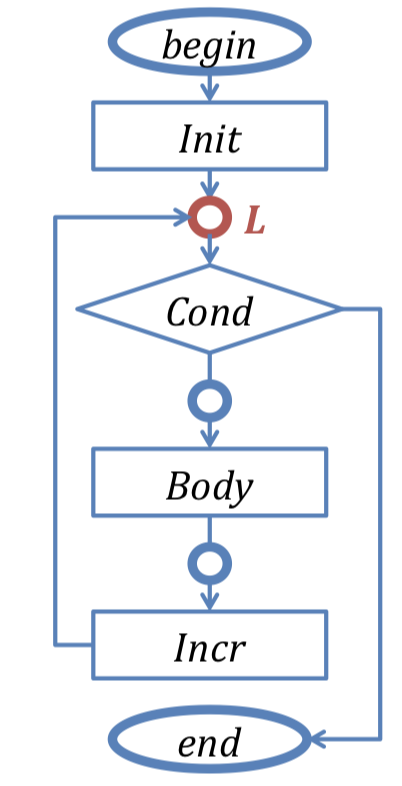
\includegraphics[width=0.3\textwidth]{img/for.png}
	\caption{Graphe d'exécution d'une boucle \texttt{for}.}
\end{figure}
\end{mydef}

\begin{mydef}
Un \emph{chemin} (\emph{path}) est une séquence exécutable
d'instructions du programme entre deux \emph{positions}.

Un \emph{chemin simple} (\emph{basic path}) est un \emph{chemin}
qui ne passe pas deux fois par la même instruction
sauf éventuellement s'il revient au point de départ,
ce qui en fait un \emph{cycle}.

Un ensemble de \emph{points de coupe} est
un ensemble de \emph{positions} du programme
tel que toutes les boucles contiennent au moins un \emph{point de coupe}.
Les chemins entre points de coupe sons des \emph{chemins simples}.
Plusieurs points de coupe sont possibles.
\end{mydef}

Les \emph{conditions} dans les instructions du programme
deviennent des \emph{assomptions} dans les chemins simples:
\begin{align}
@L1\ &\textbf{if}\ C\ \{S1\}\ \textbf{else}\ \{S2\}\ @L2\\
\rightarrow &@L1\ \textbf{assume}\ C;\ S1\ @L2\\
&@L1\ \textbf{assume}\ \lnot C;\ S2\ @L2\\&\\
@L1\ &\textbf{while}\ C\ \{S1\}\ @L2\\
\rightarrow &@L1\ \textbf{assume}\ C;\ S\ @L2\\
&@L1\ \textbf{assume}\ \lnot C;\ @L2
\end{align}
\begin{figure}[H]
	\centering
	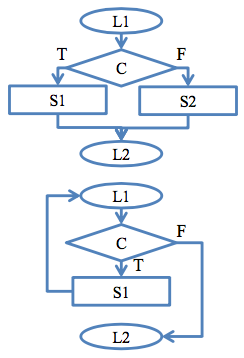
\includegraphics[width=0.4\textwidth]{img/simplegraph.png}
	\caption{Graphes d'exécution
	pour les boucles \inlinedafny{if} et \inlinedafny{while}.}
\end{figure}

L'expression \inlinedafny{assume C;} est équivante à dire que
l'exécution ne s'exécute que si $C$ est vrai.
On assume que $C$ est vrai et on ignore les exécutions où $C$ est faux.
Pour faire la preuve en \emph{avant},
on utilise la règle de l'\inlinedafny{assume} en avant:
$[P]$ \textbf{assume} $C;\ [P \land C]$.
Pour la preuve en \emph{arrière},
$[C \implies Q]$ \textbf{assume} $C;\ [Q]$.

Les \inlinedafny{assert} correpondent à l'absence d'erreurs à l'exécution.
Par exemple, vérifier que le diviseur ne soit pas égal à $0$
ou que l'indice d'un tableau est strictement plus petit que sa longueur.
Pour \inlinedafny{assert}, on affirme que $C$ est vrai,
donc on doit le prouver sur toutes les exécutions.
Pour faire la preuve en \emph{avant}:
\textbf{Si} $P \implies C$ \textbf{alors} $[P]$ \textbf{assert} $C$; $[P \land C]$.
Pour la preuve en \emph{arrière}:
\textbf{Si} $P \implies C$ \textbf{alors} $[P]$ \textbf{assert} $C$; $[P \land C]$.

Pour conclure, on peut dire qu'un chemin simple
peut se composer des instructions suivantes:
\begin{itemize}
	\item affectation $V \coloneqq E$;
	\item \inlinedafny{assume} $C$;
	\item \inlinedafny{assert} $C$;
\end{itemize}

\subsection{Calcul WP}
Pour faire la preuve des chemins simples en arrière
nous utiliserons la forme $[F[Q]]\ S\ [Q]$.
Nous obtenons alors:

\noindent $[Q[V:=E]]\ V \coloneqq E;\ [Q]$\\
$[C \implies Q]$ \textbf{assume} $C;\ [Q]$ \\
$[C \wedge Q]$ \textbf{assert} $C;\ [Q]$

La \emph{weakest precondition},
notée $\weakest(S,Q)$,
est la \emph{plus faible précondition} de $S$ pour $Q$.
Cela veut dire que $Q$ est vrai après $S$
si et seulement si $\weakest(S, Q)$ est vrai avant $S$.
Donc, nous pouvons noter que
$[P]\ S\ [Q]$ si et seulement si $P \implies \weakest(S,Q)$:
afin de prouver la validité de notre précondition,
nous devons montrer que celle-ci implique toujours la plus faible précondition.

On peut calculer $\weakest(S,Q)$ pour tout chemin simple $S$.
Les règles de calcul de $\weakest$ en arrière:
\begin{itemize}
	\item $[Q[V:=E]]\ V \coloneqq E;\ [Q] \implies \weakest(V \coloneqq E;, Q) = Q[V \coloneqq E]$
	\item $[C \implies Q]$ \textbf{assume} $C;\ [Q] \implies \weakest( \textbf{assume}\ C;, Q) = C \implies Q$
	\item $[C \wedge Q]$ \textbf{assert} $C;\ [Q] \implies\ wp(\textbf{assert}\ C;, Q) = C \land Q$
	\item Si $[P]\ S1\ [R]$ et $[R]\ S2\ [Q]$,
	alors $[P]\ S1\ S2\ [Q] \implies \weakest(S1\ S2;, Q) = \weakest(S1, \weakest(S2,Q))$
\end{itemize}

\subsection{Méthode des assertions inductives}
Pour prouver la \emph{correction partielle} de $[P]\ S\ [Q]$,
on choisit un ensemble de points de coupe $L_1,\ldots, L_n$.
Ensuite, on associe une assertion $P_i$ à chaque point de coupe $L_i$
et pour chaque \emph{chemin simple} $@L_i\ S\ @L_j$,
on va prouver $[P_i]\ S\ [P_j]$.

Si $[P_i]\ S_{ij}\ [P_j]$ est valide
pour tout \emph{chemin simple} $@L_i\ S_{ij}\ @L_j$,
alors $[P_i]\ S_{ij} \ldots S_{k\ell}\ [P_\ell]$ est valide
pout tout \emph{chemin} $@L_i\ S_{ij} \ldots S_{k\ell}\ @L_\ell$.
En particulier, $[\mathrm{Pre}]\ S\ [\mathrm{Post}]$
est valide pour le \emph{programme entier} $@\mathrm{Pre}\ S\ @\mathrm{Post}$.

\subsection{Méthode des ensembles bien-fondés}
Pour prouver la \emph{correction totale} de $[P]\ S\ [Q]$:
\begin{enumerate}
	\item On applique la \emph{méthode des assertions inductives}.
	\item Ensuite, on choisit un sous-ensemble des points de coupe
	$\{L_1', \ldots ,L_m'\}$,
	tel que chaque boucle contient au moins un $L_i'$.
	\item On associe un \emph{variant} $V_i$
	à chaque point de coupe $L_i'$.
	\item Pour chaque \emph{chemin simple} $@L_i'\ S\ L_j'$,
	on prouve $[P_i \land V_i = v_0]\ S\ [V_j < v_0]$.
\end{enumerate}

Un \emph{variant} est une expression dont la valeur
est dans un domaine bien-fondé
pour la relation considérée\footnote{C'est-à-dire
qu'il n'y a pas de chaînes décroissantes infinies.}.

Si $[P_i \land V_i = v_0]\ S\ [V_j < v_0]$ est valide
pour tout \emph{chemin simple} $@L_i'\ S_{ij}\ @L_j'$,
alors $[P_i \land V_i = v_0]\ S_{ij} \ldots S_{k\ell}\ [V_l < v_0]$ est valide
pour tout chemin $@L_i'\ S_{ij} \ldots S_{kl}\ @L_\ell'$.
En particulier, $[P_i \land V_i = v_0]\ S_{ij} \ldots S_{ki} \ [V_i<v_0]$
est valide pour tout cycle $@L_i'\ S_{ij} \ldots S_{ki}\ @L_i'$.
Il ne peut donc pas y avoir d'éxecution infinie qui boucle sur $@L_i$.
Cela veut dire que la programme se termine.
Le variant sert donc à prouver la terminaison du programme.

\section{Procédures}
\subsection{Abstraction procédurale}
\begin{mydef}[Abstraction]
\emph{Abstraire} un fragment de programme,
c'est l'utiliser pour son effet, indépendamment de son implémentation,
comme un nouvel opérateur du langage.
C'est-à-dire qu'on connait
le nom, l'interface et les spécifications de la procédure,
mais on ne regarde pas son code.

L'abstraction par \emph{paramétrage}
généralise sur le traitement des données
mais ignore les données particulières.
L'abstraction par \emph{spécification} généralise sur l'effet du programme
mais ignore les implémentations particulières.
\end{mydef}

\subsubsection{Bénéfices de l'abstraction}
L'abstraction a plusieurs bénéfices, regroupés sous le nom de \emph{modularité}:
\begin{itemize}
	\item la \emph{localité}: on peut lire ou écrire
	l'implémentation d'une abstraction
	sans devoir consulter l'implémentation des abstractions qu'elle utilise;
	\item la \emph{modifiabilité}: on peut modifier
	l'implémentation d'une abstraction
	sans modifier l'implémentation des abstractions qui l'utilisent.
\end{itemize}

\subsubsection{Déclaration de procédure}
On déclare la procédure de la façon suivante:
\begin{lstlisting}[mathescape]
procedure F(V$_1$:T$_1$,$\ldots$,V$_n$:T$_m$):T
	pre P$_F$
	post Q$_F$
{S}
\end{lstlisting}
où
\begin{itemize}
	\item \lstinline|F| est le \emph{nom} de la procédure (identifiant);
	\item \lstinline|V|$_1,\ldots,$\lstinline|V|$_n$
	sont les \emph{paramètres} (variables);
	\item \lstinline|T|$_1,\ldots,$\lstinline|T|$_n$, \lstinline|T|
	sont les \emph{types};
	\item \lstinline|P|$_F$, \lstinline|Q|$_F$
	sont les \emph{spécifications} (assertions) et
	\item \lstinline|S| est le \emph{corps} (instructions).
\end{itemize}
Les spécifications respectent
l'abstraction en termes de l'interface \lstinline|F|
pour les paramètres et le résultat.
Les types sont des spécifications
qui sont supportées dans le langage de programmation.

\subsubsection{Résultats d'une procédure}
En général, une procédure peut avoir \emph{plusieurs paramétres}
et retourner \emph{plusieurs résultats}.
Dans la suite du cours, on présente des procédures (\lstinline|F(V) {S}|)
avec un seul paramètre et qui retournent un seul résultat ($U \coloneqq F(E)$).
On peut tout généraliser à plusieurs valeurs et considérer $V$, $E$
comme des tuples: $V=(V_1,\ldots,V_n)$ et $E=(E_1,\ldots,E_m)$.

Le résultat de la procédure est une variable distinguée \emph{result}.
L'axiome du \inlinedafny|return| est
\begin{align}
&[Q[E/result]]\ \texttt{return E}\ [Q]\\
&\weakest(\texttt{return E}, Q) = Q[E/result]
\end{align}
\begin{myrem}
	En \textsc{Dafny} on n'a pas de \emph{result};
	il faut créer une variable qui représente le résultat.
\end{myrem}

Pour faire la preuve de la procédure ci-dessus (dans le cas non typé),
dans $S$ on remplace \texttt{return E;} par \texttt{result $\coloneqq$ E}.
Ensuite, on prouve $[P_F]\ S\ [Q_F]$
par exemple par assertions inductives et ensembles bien-fondés.

\subsection{Procédure pures}
On décompose les expressions en expressions atomiques.
\begin{myexem}
\texttt{y := exp(x, 10) / 2} devient \texttt{var u := exp(x, 10); y := u / 2},
où \texttt{u} est une \emph{variable fraîche}
qui n'existe pas encore dans le programme.
\end{myexem}

\begin{mydef}
Une \emph{procédure pure}
est une procédure où les variables non locales ne sont \emph{pas modifiées}
par les instructions de la procédure.
Les paramètres sont passés \emph{par valeur} et ne sont donc pas modifiés.
Dans ce cas-là, la précondition $P_F$ porte uniquement
sur les paramètres de la procédure
et la postcondition $Q_F$ sur les paramètres (non modifiés) et le résultat:
\begin{lstlisting}[mathescape]
procedure F(V$_1$,$\ldots$,V$_n$)
	pre P$_F$[V$_1$,$\ldots$,V$_n$]
	post Q$_F$[V$_1$,$\ldots$,V$_n$, result]
{S}
\end{lstlisting}
\end{mydef}

\subsubsection{Appel de procédure}
Pour une procédure pure, si on a prouvé $[P_F]\ S\ [Q_F]$,
alors on peut remplacer \texttt{U $\coloneqq$ F(E);}
par \inlinedafny{assert P$_F$[E/V]; assume Q$_F$[E/V,U/result];}.

La régle de la procédure se note:
\begin{center}
Pour une procédure $F(V)\ \{S\}$,\\ \medskip
\begin{tabular}{ll}
	Si & $[P_F]\ S\ [Q_F]$,\\\\
	alors & $\Big[P_F[E/V]\Big]$\\
	& \texttt{U $\coloneqq$ F(E);}\\
	& $\Big[Q_F[E/V, U/result]\Big]$
\end{tabular}
\end{center}
ou, de manière équivalente:
\begin{center}
Pour une procédure $F(V)\ \{S\}$,\\ \medskip
\begin{tabular}{ll}
	Si & $\big[P_F[V]\big]\ S\ \big[Q_F[V, result]\big]$,\\\\
	alors & $\Big[P_F[E]\Big]$\\
	& \texttt{U $\coloneqq$ F(E);}\\
	& $\Big[Q_F[E,U]\Big]$
\end{tabular}
\end{center}

Pour une procédure $F(V)\ \textbf{pre}\ P_F\ \textbf{post}\ Q_F\ \{S\}$
et pour un appel $U \coloneqq F(E)$,
on a:
\begin{align}
	&\Big[P_F[E/V] \land \big(Q_F[E/V, U/result] \implies Q\big)\Big]\\
	&\texttt{assert P$_F$[E/V];}\\
	&\Big[Q_F[E/V, U/result] \implies Q\Big]\\
	&\texttt{assume Q$_F$[E/V, U/result];}\\
	&\Big[Q\Big]
\end{align}
à condition
\begin{itemize}
	\item que la précondition $P_F$ soit vraie en $E$ et
	\item que la postcondition $Q_F$ soit vraie en $E$ et $U$ implique $Q$.
\end{itemize}

\subsection{Procédures avec effet}
Les procèdures non pures peuvent modifier des variables non locales
et permettent de transmettre des paramètres \emph{par référence}:
\textbf{procedure} $F(V)$ \textbf{pre} $P_F$
\textbf{post} $Q_F$ \textbf{modifies} $V\ \{S\}$.
$S$ modifie $V$: la valeur de $V$ est différente
à l'entrée et à la sortie de $S$.

En \java,
\begin{itemize}
	\item tous les types objets (non primitifs) sont transmis par référence,
	y compris les tableaux.
	\item \lstinline[language=Java]|this| est le paramètre
	\emph{par référence} implicite de toutes les méthodes d'instance.
	\item Un objet \emph{immuable} ou qui n'est \emph{pas modifié}
	peut être considéré comme passé \emph{par valeur}.
\end{itemize}

Pour une procédure avec effet, si on a prouvé $[P_F]\ S\ [Q_F]$,
alors on peut remplacer \texttt{U $\coloneqq$ F(A);} par
\begin{dafny}[mathescape]
assert P$_F$[A/V];
A := a$_1$;
assume Q$_F$[A/V, U/result];
\end{dafny}
où \inlinedafny|a|$_1$ est une variable auxiliaire fraîche
qui représente la valeur de \inlinedafny|A| à la sortie de $S$.

Règle de la procédure avec effet:
\begin{center}
Pour une procédure $F(V)\ \{S\}$:\\ \medskip
\begin{tabular}{ll}
	Si & $[P]\ S\ [Q]$,\\\\
	alors & $\Big[P[A/V]\Big]$\\
	& \texttt{U $\coloneqq$ F(A);}\\
	& $\Big[Q[A/V,U/result]\Big]$
\end{tabular}
\end{center}

Pour faire la preuve pour la procédure avec effet suivante:
\textbf{procedure} $F(V)$ \textbf{pre} $P_F \land V = V_0$
\textbf{post} $Q_F[v_0]$ \textbf{modifies} $V$
et pour un appel \texttt{U $\coloneqq$ F(A)}, on a:
\begin{align}
	&\Big[P_F[E/V] \land \big(Q_F[a_1/V, U/result] \implies Q[a_1/A]\big)\Big]\\
	&\texttt{assert P$_F$[A/V];}\\
	&\Big[Q_F[a_1/V, U/result] \implies Q[a_1/A]\Big]\\
	&\texttt{A := a$_1$;}\\
	&\Big[Q_F[A/V, U/result] \implies Q\Big]\\
	&\texttt{assume Q$_F$[A/V, U/result];}\\
	&\Big[Q\Big]
\end{align}

Pour faire la preuve avec des variables auxiliaires
pour une procédure avec effet,
on doit introduire une \emph{variable auxiliaire libre} $v_0$.
Donc, pour prouver $[P]\ \texttt{U := F(A);}\ [Q]$,
on a $[P_F \land V=v_0]\ S\ \big[Q_F[v_0]\big]$ pour tout $v_0$.
On peut poser $A = v_0$.

\subsection{Procédures récursives}
Régle de la procédure récursive:
on \emph{suppose} que les \emph{appels} soient corrects,
puis on \emph{prouve} que le \emph{corps} est correct.
\begin{center}
Pour une procédure récursive $F(V)\ \{S\}$:\\ \medskip
\begin{tabular}{lll}
Si & si & $\Big[P_F[E/V]\Big]$,\\
&& \texttt{U $\coloneqq$ F(E);}\\
&& $\Big[Q_F[E/V, U/result]\Big]$\\\\
& alors & $[P_F]\ S\ [Q_F]$,\\\\
alors & \multicolumn{2}{l}{$[P_F]\ S\ [Q_F]$}\\\\
et donc & \multicolumn{2}{l}{$\Big[P_F[E/V]\Big]$}\\
& \multicolumn{2}{l}{\texttt{U $\coloneqq$ F(E);}}\\
& \multicolumn{2}{l}{$\Big[Q_F[E/V, U/result]\Big]$}
\end{tabular}
\end{center}

Par induction complète sur la profondeur maximale des appels récursifs,
on peut justifier cette règle:
$R[n]$ est défini comme \og si la profondeur maximale
des appels récursifs de $F(E)$ est $n$, alors
$\big[P_F[E/V]\big]\ \texttt{U := F(E);}\ \big[Q_F[E/V, U/result]\big]$\fg.
On pose $R[k]$ pour $k<n$, on prouve $R[n]$ (via $[P]\ S\ [Q]$)
et on conclut que $R[n]$ est vrai pour tout $n$.

Pour une procédure récursive \textbf{procedure} $F(V)$ \textbf{pre} $P_F$
\textbf{post} $Q_F$\ \{S\},
dans la preuve de $[P_F]\ S\ [Q_F]$,
on peut remplacer les appels récursifs $F(E)$ par \textbf{assert} $P_F[E/V]$;
\textbf{assume} $Q_F[E/V, U/result];$.

\subsubsection{Correction totale}
Pour les procédures récursives, il peut y avoir récursion infinie.
On définit un variant sur les paramètres de la procédure;
\textbf{procedure} $F(V)$ \textbf{pre} $P_F$
\textbf{post} $Q_F$ \textbf{variant} $Z_F\ \{S\}$.
Le variant doit décroître pour les appels récursifs de $F$ dans $S$.

La règle de la correction totale pour une procédure récursive $F(V)\ \{S\}$:
\begin{center}
Pour une procédure récursive $F(V)\ \{S\}$:\\ \medskip
\begin{tabular}{lll}
Si & si & $\Big[P_F[E/V] \land Z[E/V] < z_0\Big]$,\\
&& \texttt{U $\coloneqq$ F(E);}\\
&& $\Big[Q_F[E/V, U/result]\Big]$\\\\
& alors & $[P_F \land Z=z_0]\ S\ [Q_F]$,\\\\
alors & \multicolumn{2}{l}{$[P_F]\ S\ [Q_F]$}\\\\
et donc & \multicolumn{2}{l}{$\Big[P_F[E/V]\Big]$}\\
& \multicolumn{2}{l}{\texttt{U $\coloneqq$ F(E);}}\\
& \multicolumn{2}{l}{$\Big[Q_F[E/V, U/result]\Big]$}
\end{tabular}
\end{center}

Pour une procédure récursive \textbf{procedure} $F(V)$ \textbf{pre} $P_F$
\textbf{post} $Q_F$ \textbf{variant} $Z_F\ \{S\}$,
dans la preuve de $[P_F \land Z = z_0]\ S\ [Q_F]$,
on peut remplacer les appels récursifs $F(E)$ par
\textbf{assert} $P_F[E/V] \land Z[E/V] < z_0;$
\textbf{assume} $Q_F[E/V, U/result];$.

\section{Structure de données}
\subsection{Types de données}
\begin{mydef}[Type de données]
Un \emph{type de données} (\emph{data type})
est défini par des \textbf{données} et des \textbf{opérations}.
Soit \(D_T\) l'ensemble des \textbf{valeurs} (objets) possibles,
et \(OP_T\) l'ensemble des \textbf{opérations} (procédures) possibles;
On écrit alors \(T \equiv (D_T, OP_T)\).
Dans la procedure $F(V_1:T_1,\ldots,V_n:T_n):T'$
où les paramètres $T_1,\ldots,T_n$ peuvent être de type $T$,
ainsi que le résultat $T'$.
\end{mydef}

\subsubsection{Opérations avec effets}
\begin{mydef}[Opérations avec effet]
Les \emph{opérations avec effets} sont les opérations
qui modifient les paramètres, passés \textbf{par référence}.
Il s'agit alors de procédures \textbf{non pures}.
\end{mydef}

\subsubsection{Types d'opérations}
Pour un type $T \equiv (D_T, OP_T)$,
une opération $F(V_1:T_1,\ldots,V_n:T_n):T' \in OP_T$
\begin{itemize}
	\item est un \emph{producteur} de $T$ si et seulement si $T'=T$;
	\item est un \emph{créateur} de $T$
	si et seulement si
	$T'=T$ et $T_1,\ldots,T_n \ne T$;\footnote{Un créateur
	est donc également un producteur.}
	\item est un \emph{observateur} de $T$
	si et seulement si $T' \ne T$, avec $T'$ non vide;
	\item est un \emph{modificateur} de $T$
	si et seulement si $T'$ est vide;
	\item est un \emph{mutateur} de $T$ si et seulement si $T_i = T$
	et $F$ modifie $V_i$.
\end{itemize}

\subsubsection{Type immuable}
\begin{mydef}[Type immuable]
Un type $T$ est \emph{immuable} s'il n'a \textbf{aucun mutateur};
c'est-à-dire qu'aucune opération ne modifie de paramétre de type $T$.
C'est une \textbf{propriété du type}, pas de son implémentation.
Grâce à cette propriété on peut \textbf{partager} les valeurs.
Par contre, on doit créer et détruire plus d'objets.
\end{mydef}

\subsubsection{Enregistrements}
\begin{mydef}[Enregistrement]
Les \emph{enregistrements} peuvent être décrits comme
\texttt{type} \(T = {F_1:T_1,\ldots,F_n:T_n}\).
Il s'agit d'un type \textbf{produit}:
$D_T = D_{T_1} \times \cdots  \times D_{T_n}$.
Les opérations possibles sur un enregistrement sont
\begin{itemize}
	\item les \textbf{producteurs},
	typiquement les constructeurs;
	\item les \textbf{observateurs},
	typiquement les accesseurs;
	\item les \textbf{modificateurs},
	typiquement les fonctions \texttt{set}.
\end{itemize}
\end{mydef}

\subsubsection{Unions}
\begin{mydef}[Union]
Les \emph{unions} peuvent être décrites comme
\texttt{type} $T = F_1:T_1 \mid \cdots \mid F_n:T_n$.
Il s'agit d'un type \textbf{somme}: $D_T = D_{T_1} + \cdots + D_{T_n}$.
Les opérations possibles sur une union sont
\begin{itemize}
	\item les \textbf{producteurs},
	typiquement les constructeurs;
	\item les \textbf{observateurs},
	typiquement les accesseurs.
\end{itemize}
\end{mydef}

\subsection{Types de données inductifs}
\subsubsection{Type inductif}
\begin{mydef}[Type inductif]
La forme générale d'un \emph{type de données inductif} est
\texttt{datatype} $T = G_1(F_{11}:T_{11},\ldots) \mid \cdots  \mid G_n(F_{n1}:T_{n1},\ldots)$.
Un \emph{type inductif} ou \emph{algébrique}
est une somme de produits (une union d'enregistrements)
où $G_1,\ldots,G_n$ sont les \textbf{générateurs} du type $T$.
\end{mydef}

Des exemples de types inductifs sont
\begin{itemize}
	\item les \textbf{énumérations};
	\item les \textbf{unions};
	\item les \textbf{enregistrements};
	\item les \textbf{grammaires};
	\item les \textbf{entiers naturels}.
\end{itemize}
Les opérations possibles sur un type inductif sont
\begin{itemize}
	\item les \textbf{producteurs},
	typiquement les constructeurs;
	\item les \textbf{observateurs},
	typiquement les accesseurs;
	\item les \textbf{modificateurs},
	typiquement les fonctions \texttt{set}.
\end{itemize}

\subsubsection{Filtrage}
\begin{mydef}[Filtrage]
On définit l'instruction de \emph{filtrage} (\emph{pattern matching})
\texttt{match} $E$ \{\texttt{case} $M_1 \implies S_1 \ldots$
\texttt{case} $M_k \implies S_k$\}.
où $M_1,\ldots,M_k$ sont des \textbf{motifs} (\textbf{patterns})
constitués de générateurs et de variables.
Les variables de $M_1,\ldots,M_k$ apparaissent dans $S_1,\ldots,S_k$.
Le filtrage consiste à exécuter le premier $S_i$
tel que la valeur de $E$ correspond avec le motif \(M_i\).
\end{mydef}

\paragraph{Filtrage primitif}
On peut également définir l'instruction de \emph{filtrage primitif}:
\begin{lstlisting}
match E {
	case G1(V1,...) => S1
	...
	case Gk(Vk,...) => Sk
}
\end{lstlisting}
où $G_1,...,G_k$ sont tous les générateurs du type de $E$.

\begin{myprop}
	Le filtrage général peut se réduire en filtrage primitif.
	On a la \emph{règle du filtrage primitif (version arrière)}:
	\begin{center}
	\begin{tabular}{ll}
	Si & $[P_i]\ S_i\ [Q]$, pour $i = 1, \ldots, n$,\\
	alors & $\left[\bigwedge_{i=1}^n(E = G_i(V_i) \implies P_i)\right]$\\
	& \texttt{match} E \{\\
	& \texttt{        case} $G_1(V_1) \implies S_1$\\
	& \texttt{        ...}\\
	& \texttt{        case} $G_n(V_n) \implies S_n$\\
	& \}\\
	& $[Q]$
	\end{tabular}
	\end{center}
\end{myprop}

\subsubsection{Domaine d'un type inductif}
Définissons le type
\texttt{datatype Tree = leaf(i: Int) | node(left: Tree, right: Tree)}.
L'\textbf{algèbre de termes} des générateurs de \emph{Tree} est
\begin{align}
\dtree^{0} &= \emptyset\,,\\
\dtree^{k+1} &= \dtree^{k} \cup {\texttt{leaf}(i) \mid i \in D_{\texttt{Int}}} \cup {\texttt{node}(l, r) \mid l, r \in \dtree^{k}}\,,\\
\dtree &= \bigcup_k \dtree^{k}\,.
\end{align}
Il faut au moins un créateur, sinon $\dtree = \emptyset$.

\subsubsection{Induction bien-fondée pour les types inductifs}
Soit la relation $\letree$ définie sur $\dtree$ telle que
$d \letree d'$ si et seulement si $d$ est un \textbf{sous-terme} de $d'$.
La relation $\letree$ est \textbf{bien-fondée} sur $\dtree$.
Pour tout type inductif $T$, $<_T$ est bien-fondée sur $D_T$.

$d \prectree d'$ si et seulement si
$d$ est un \textbf{sous-terme direct} de $d'$.
Pour tout type inductif $T, \prec_T$ est \textbf{bien-fondée} sur $D_T$.

\subsubsection{Induction structurelle}
Pour un type inductif $T$, l'induction structurelle sur $T$
est équivalente à l'induction bien-fondée sur \(<_T\):
\begin{center}
\begin{tabular}{lll}
Si & si & $P[y]$ est vrai pour tout sous-terme $y$ de $x$,\\
& alors & $P[x]$ est vrai,\\
alors & \multicolumn{2}{l}{$P[x]$ est vrai pour tout $x$.}\\\\
\end{tabular}
\end{center}

\subsection{Procédures par induction structurelle}
\begin{mydef}[Procédure définie par induction structurelle]
Pour un type inductif $T$,
pour une procédure récursive $F(V: T,\ldots): T'\ \{S\}$,
$F$ est \emph{définie par induction structurelle} sur $T$
si pour tous les appels récursifs $F(E,\ldots)$ dans $S$,
$E$ est un sous-terme de $V$.

Si $F$ est définie par induction structurelle,
alors $F$ se termine \textbf{toujours}.
\end{mydef}

\section{Abstraction sur les données}
\subsection{Abstraction et représentation}
Seuls certains types sont \textbf{directement supportés}
par le langage de programmation.
En général, on doit \textbf{construire une représentation} du type désiré
sur base de types primitifs du language.
On représente un \textbf{type abstrait} $A$ par un \textbf{type concret} $T$.

\begin{mydef}[Type abstrait]
	Un \emph{type abstrait} $A$ est une \textbf{structure quelconque}.
	Il est exprimé en mathématique (et est donc libre).
\end{mydef}

\begin{mydef}[Type concret]
	Un \emph{type concret} $T$ est un
	\textbf{type du langage} de programmation
	exprimé \textbf{dans le langage} de programmation.
\end{mydef}

On veut représenter un \textbf{type abstrait} $A=(D_A, OP_A)$
sur base d'un \textbf{type concret} $T=(D_T, OP_T)$;
on doit donc
\begin{itemize}
	\item représenter les \textbf{valeurs abstraites}
	$a \in D_A$ en \textbf{valeurs concrètes} $d \in D_T$ et
	\item implémenter les \textbf{opérations abstraites}
	$op \in OP_A$ sous forme de
	\textbf{procédures sur les valeurs concrètes}.
\end{itemize}

\subsection{Fonction d'abstraction}
\begin{mydef}[Fonction d'abstraction]
	Soit un type \(A = (D_A, OP_A)\) représenté par \(T = (D_T, OP_T)\).
	La \emph{fonction d'abstraction} du type $A$,
	$\absf_A \colon D_T \to D_A$,
	où $a = \absf_A(d) \in D_A$, est la valeur de $A$
	\textbf{représentée par} $d \in D_T$.
	La fonction $\absf_A$ est \textbf{partielle}
	car $\absf_A(d)$ n'est pas défini
	si $d$ n'est pas une représentation valide d'une valeur de $A$.
	La fonction $\absf_A$ n'est \textbf{pas injective}
	car il peut y avoir plusieurs représentations
	$\absf_A(d') = \absf_A(d'') = a$ de la même valeur $a$ de $A$.
\end{mydef}

\subsection{Relation d'équivalence}
\begin{mydef}[Relation d'équivalence]
	Soit un type \(A = (D_A, OP_A)\) représenté par \(T = (D_T, OP_T)\).
	La \emph{relation d'équivalence} du type $A$,
	\(\sim_A\), est définie par
	\begin{align}
		\sim_A &\colon D_T \times D_T \to \mathrm{Bool}\,,\\
		d \sim_A d' &\equiv \absf_A(d) = \absf_A(d')\,.
	\end{align}
	$d \sim_A d'$ signifie donc que \(d, d' \in D_T\) représentent
	la \textbf{même valeur} de \(A\).
	La relation \(\sim_A\) détermine
	des \textbf{classes d'équivalence} dans \(D_T\).
\end{mydef}

\subsubsection{Congruence}
\begin{mydef}[Congruence]
Une opération $F$ est \emph{congruente} par rapport à l'équivalence $\sim$
si et seulement si des \textbf{arguments équivalents}
donnent des \textbf{résultats équivalents}.
Pour \(F(V: T, \ldots)\),
\(d \sim d' \implies F(d, \ldots) \sim F(d', \ldots)\).

Toutes les opérations de l'abstraction
\textbf{doivent être congruentes} par rapport à $\sim$;
\begin{itemize}
	\item c'est le cas si elles représentent
	correctement une opération abstraite,
	\item sinon c'est une violation de l'abstraction.
\end{itemize}

Si on a une \textbf{opération abstraite} $f \colon D_A \to D_A$
et une \textbf{procédure} $F(V: T): T$ qui représente $f$
(telle que \(\absf(F(d)) = f(\absf(d))\)) alors $F$ est \emph{congruente}.
\end{mydef}

\subsection{Invariant de représentation}
\begin{mydef}[Invariant de représentation]
	Soit un type \(A = (D_A, OP_A)\) représenté par \(T = (D_T, OP_T)\).
	L'\emph{invariant de représentation} (\emph{rep-invariant}) du type $A$,
	\(\ok_A\), est défini par
	\begin{align}
		\ok_A &\colon D_T \to \mathrm{Bool}\,,\\
		\ok_A(d) &\equiv (\absf_A(d) \textnormal{ est défini})\,.
	\end{align}
	$\ok_A(d)$ signifie donc que
	\(d\) représente une \textbf{valeur valide} de $A$.
\end{mydef}

\subsection{Spécification}
Grâce à ces concepts, on peut faire de la spécification.
Pour spécifier la structure d'un type de données,
on doit définir l'abstraction \(\absf\) et le rep-invariant \(\ok\).
Pour spécifier les opérations,
on doit utiliser ceux-ci pour donner les pré-/postconditions,
ainsi que les effets.

\subsection{Abstraction en orienté-objets}
L'\emph{abstraction des données} est à la base
de la programmation orientée-objets:
\begin{itemize}
	\item un \textbf{type abstrait} est représenté par une \textbf{classe};
	\item la \textbf{représentation} est équivalente
	aux \textbf{variables d'instance} de la classe;
	\item les \textbf{opérations abstraites} sont représentées
	par les \textbf{méthodes} de la classe;
	\item toutes les méthodes ont un
	\textbf{paramètre implicite}\footnote{Par référence et modifiable.},
	\texttt{this}.
\end{itemize}

\subsubsection{Préservation}
\paragraph{Préservation du rep-invariant}
La représentation de $A$ par $T$ \emph{préserve le rep-invariant}
si et seulement si
\begin{itemize}
	\item tous les \textbf{producteurs} $F(V:T,\ldots):T\ \{S\}$
	préservent $\ok$: $[\ok(V)]\ S\ [\ok(result)]$;
	\item tous les \textbf{mutateurs} $F(V:T,\ldots):T'\ \{S\}$
	préservent $\ok$: $[\ok(V)]\ S\ [\ok(V)]$.
\end{itemize}

\begin{myprop}[Préservation du rep-invariant]
Si tous les \textbf{producteurs} et \textbf{mutateurs} de $OP_T$
\textbf{préservent} $\ok$ et
seules les \textbf{opérations} de $OP_T$ sont utilisées
pour produire des valeurs de $T$,
alors toutes les valeurs de $T$ \textbf{satisfont} $\ok$.
\end{myprop}

\paragraph{Préservation de la représentation}
Pour assurer la \textbf{modularité},
il faut \textbf{préserver} et \textbf{masquer} la \emph{représentation}.
\begin{itemize}
	\item La \emph{représentation} n'est \textbf{pas modifiable
	en dehors} de l'implémentation de l'abstraction.
	Cela implique la \textbf{localité}:
	on peut \textbf{raisonner} sur l'implémentaion indépendamment du reste.
	\item La \emph{représentation} n'est \textbf{pas visible
	en dehors} de l'implémentation de l'abstraction.
	Cela implique la \textbf{modifiabilité}:
	on peut \textbf{modifier} l'implémentation indépendamment du reste.
\end{itemize}

\paragraph{Préservation en orienté-objets}
La \textbf{programmation orientée-objets} permet
la préservation de la représentation.
\begin{itemize}
	\item L'\textbf{encapsulation} rassemble
	la structure qui représente l'abstraction et
	les opérations associées
	en une \textbf{classe} qui représente le type abstrait.
	\item Les \textbf{modificateurs de visibilité}
	limitent les opérations accessibles et
	permettent de \textbf{préserver} et \textbf{masquer} la représentation.
\end{itemize}

Si la représentation est accessible en dehors de l'implémentation,
on dit que l'implémentation \textbf{expose} la représentation.
C'est une \textbf{erreur de conception}.
Quelque causes possibles sont
\begin{itemize}
	\item une faille de \textbf{visibilité};
	\item une \textbf{référence exportée};
	\item une \textbf{référence importée}.
\end{itemize}

\subsubsection{Effets bienveillants}
Un type abstrait \textbf{mutable} a forcément
des \textbf{opérations avec effet} (mutateurs).

Un type abstrait \textbf{immuable} \textbf{peut} avoir
des \textbf{opérations avec effet}.
\begin{mydef}[Effet bienveillant]
	Un \emph{effet bienveillant} est un effet
	qui n'est pas visible en dehors de l'abstraction.
\end{mydef}

\subsubsection{Représentation}
\paragraph{Représentation de l'équivalence}
On veut représenter l'\textbf{égalité} du type abstrait
par une \textbf{procédure} $\texttt{eq}(d,d')$,
ce qui revient à implémenter \textbf{équivalence} \(d \sim d'\).
Si on a \(\absf\) sous forme logique,
on peut spécifier et prouver
\begin{lstlisting}[mathescape]
procedure eq(d: T, d': T): Bool
pre ok(d) $\land$ ok(d')
post result $\iff$ abs(d) = abs(d')
{...}
\end{lstlisting}
et donc \texttt{eq} est congruente par rapport à $\sim$.

\paragraph{Représentation canonique}
\begin{mydef}[Représentation canonique]
	La représentation de $A$ par $T$ est \emph{canonique}
	si toutes les valeurs abstraites ont une \textbf{représentation unique}.
	Dans ce cas, $d \sim d' \iff \absf(d) = \absf(d') \iff d = d'$.
	On peut définir \texttt{eq(d,d') \{return (d = d');\}}.
\end{mydef}

\section{Conception d'algorithmes}
\subsection{Principes de conception d'algorithmes}
\begin{mydef}[Algorithme]
Un \emph{algorithme} est une procédure pour accomplir une certaine tâche.
\end{mydef}

Quelques principes généraux pour concevoir un algorithme sont
\begin{itemize}
	\item la \textbf{décomposition en sous-problèmes};
	\item \textbf{diviser pour règner} et
	\item la \textbf{programmation dynamique}.
\end{itemize}

\subsubsection{Analyse de complexité}
Pour un problème de taille $n$,
on dit que $T(n)$ est le \textbf{temps} pour résoudre un problème de taille $n$
\textbf{dans le pire cas} et
$S(n)$ est l'\textbf{espace} pour résoudre un problème de taille $n$
\textbf{dans le pire cas}.

\subsection{Décomposition en sous-problèmes}
Soit une procédure \texttt{Prob} définie comme
\begin{lstlisting}
procedure Prob(x) pre ... post ...
{
	var x1 := Subprob1(x);
	var x2 := Subprob2(x, x1);
	return solution(x, x1, x2);
}
\end{lstlisting}

On spécifie les \texttt{Subprob}:
\begin{itemize}
	\item on \textbf{programme} et \textbf{prouve} \texttt{Prob}
	sur base des \textbf{spécifications} des \texttt{Subprob},
	indépendamment de leur code;
	\item on \textbf{programme} et \textbf{prouve} chaque \texttt{Subprob}
	sur base de ses spécifications,
	indépendamment du code de \texttt{Prob} et des autres \texttt{Subprob}.
\end{itemize}

\subsection{Diviser pour régner}
Diviser pour régner consiste à
\begin{itemize}
	\item \textbf{décomposer} un problème en sous-problèmes plus petits;
	\item \textbf{résoudre} ces sous-problèmes et
	\item \textbf{combiner} les solutions des sous-problèmes
	en une solution du problème initial.
\end{itemize}
Cette décomposition est utile si
le \textbf{gain sur la réduction} en problèmes plus petits est supérieur
au travail supplémentaire pour la \textbf{décomposition et combinaison}.

\subsubsection{Schéma}
Soit la procédure \texttt{DR} suivante:
\begin{lstlisting}
procedure DR(x)
{
	if estSimple(x) {
		return simple(x);
	} else {
		x1, ..., xk := decompose(x);
		for i := 1...k {yi := DR(xi);}
		y := compose(y1, ..., yk);
		return y;
	}
}
\end{lstlisting}
où \texttt{estSimple(x)} retourne \lstinline|true|
quand \texttt{x} est suffisamment simple,
\texttt{simple(x)} est un algorithme efficace sur les instances simples.
\texttt{decompose(x)} décompose en sous-problèmes plus simples et
\texttt{compose(y1, ..., yk)} recombine les solutions.

\begin{figure}[H]
	\centering
	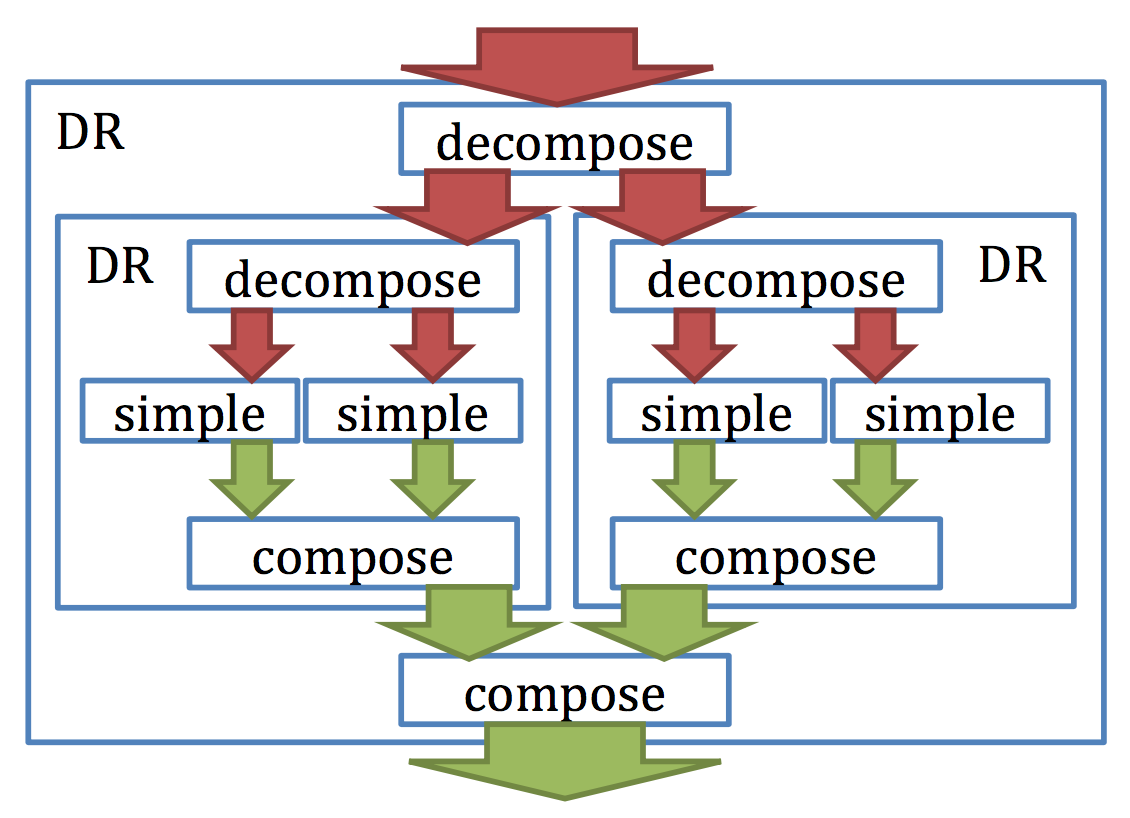
\includegraphics[width=\textwidth]{img/DR.png}
	\caption{Visualisation de la procédure \og diviser pour règner\fg.}
\end{figure}

Si \texttt{compose(x) = x}, le problème se simplie et on a
\begin{lstlisting}[mathescape]
procedure DR(x) {
	while $\lnot$estSimple(x) {
		x := decompose(x);
	}
	return simple(x);
}
\end{lstlisting}

\begin{mytheo}
	Soit $x$ de taille $n$, $x_1,\ldots, x_k$ de taille $\frac{n}{b}$
	et $g(n)$ le temps pris pas \texttt{decompose()} et \texttt{compose()},
	alors $T(n) = k T(n/b) + g(n)$.
	Si en plus, $g(n) = \Theta(n^c)$, alors
	\begin{itemize}
		\item $T(n) = \Theta(n^c)$ si $k < b^c$;
		\item $T(n) = \Theta(n^c \log n)$ si $k = b^c$;
		\item $T(n) = \Theta(n^{\log k/\log b})$ si $k > b^c$.
	\end{itemize}
\end{mytheo}

Pour passer à l'algorithme simple, il ne faut pas nécessairement attendre $n=1$;
on peut s'arrêter à $n_0$, choisi afin de minimiser $T(n)$:
\begin{itemize}
    \item $T(n) = h(n)$ si $n \le n_0$;
    \item $T(n) = k T(n/b) + g(n)$ si $n \le n_0$.
\end{itemize}
Le choix de \(n_0\) dépend de l'\textbf{implémentation}.

\subsection{Programmation dynamique}
La programmation dynamique consiste à
\begin{itemize}
	\item \textbf{décomposer} le problème en sous-problèmes;
	\item \textbf{résoudre} les sous-problèmes une seule fois
	et \textbf{mémoriser leur solutions} et
	\item \textbf{utiliser} les solutions pour la résolution du problème.
\end{itemize}
Dans ce cas on fait un compromis entre espace-temps:
on \textbf{réduit le temps} de calcul
mais on \textbf{augmente l'espace} mémoire.
La programmation dynamique est applicable lorsqu'il y a
\begin{itemize}
	\item des \textbf{sous-structures optimales}:
	la solution à un problème se \textbf{décompose} en
	solutions à des sous-problèmes et
	\item un \textbf{recouvrement des sous-problèmes}:
	la solution à un problème fait appel \textbf{plusieurs fois}
	aux mêmes sous-problèmes.
\end{itemize}

Soit \texttt{probl(x)} l'ensemble des problèmes à résoudre pour \texttt{x}.
On définit alors
\begin{itemize}
	\item \(\texttt{probl(x)} = \bigcup i : \texttt{probl}_i\texttt{(x)}\);
	\item \(\texttt{probl}_0\texttt{(x)} = \{\,\texttt{x}\,\}\);
	\item \(\texttt{probl}_{i+1}\texttt{(x)} = \bigcup \{\, \texttt{decompose(y)} \mid y \in \texttt{probl}_i\texttt{(x)}, \lnot\texttt{estSimple(x')}\,\}\);
	\item \(\texttt{problSimple(x)} = \{\,\texttt{x'} \in \texttt{probl(x)} \mid \texttt{estSimple(x')}\,\}\).
\end{itemize}

\subsubsection{Approche bottom-up}
On calcule et \textbf{mémorise les solutions}
des sous-problèmes liés au problème principal,
\textbf{à partir du problème simple} jusqu'au problème principal,
en \textbf{utilisant les solutions} des sous-problèmes déjà calculés.

\begin{lstlisting}[mathescape]
procedure PD(x)
{
	var cache := new Solution[Problem];
	forall x' $\in$ problSimple(x) { cache[x'] := simple(x'); }
	while x $\notin$ cache {
		forall x' $\in$ probl(x): decompose(x') $\subseteq$ cache {
			var x1, ..., xk := decompose(x');
			cache[x'] := compose(cache[x1], ..., cache[xk]);
		}
	}
	return cache[x];
}
\end{lstlisting}

Avec l'approche \textbf{bottom-up}, on peut réduire le coût en espace
en ne gardant que les résultats nécessaires à la suite.
Par contre on risque de calculer des sous-problèmes inutiles
et la méthode est peu naturelle.

\subsubsection{Approche top-down}
Dans un algorithme \textbf{récursif}, on \textbf{mémorise le résultat}
pour chaque sous-problème résolu et on \textbf{retourne le résultat mémorisé}
pour les appels successifs au même problème.

\begin{lstlisting}[mathescape]
var cache = new Solution[Problem];

procedure DRPD(x) {
	if x $\notin$ cache { cache[x] := DRPD1(x) ; }
	return cache[x];
}

DRPD1(x) {
	if estSimple(x){ return simple(x); }
	else {
		var x1, ..., xk := decompose(x);
		for i := 1..k { yi :=DRPD(xi); }
		return compose(y1, ..., yk);
	}
}
\end{lstlisting}

\begin{mydef}[Mémoïsation]
	La \emph{mémoïsation} est le fait de mémoriser
	les résultats d'une fonction.
\end{mydef}

Avec l'approche \textbf{top-down}, on résout uniquement
les sous-problèmes nécessaires.
Par contre, on garde en mémoire tous les sous-problèmes résolus.

\section{Preuve automatique}
\subsection{Preuve automatique de programme}
Le \textbf{programmeur} spécifie les pré-/postconditions, les invariants,
les variants et les effets.
Le \textbf{prouveur de programmes} considère chaque procédure séparément,
décompose en chemins simples et calcule la plus faible précondition pour chacun.
Le \textbf{prouveur d'assertions} fait la preuve pour chaque chemin simple.

\begin{figure}[H]
	\centering
	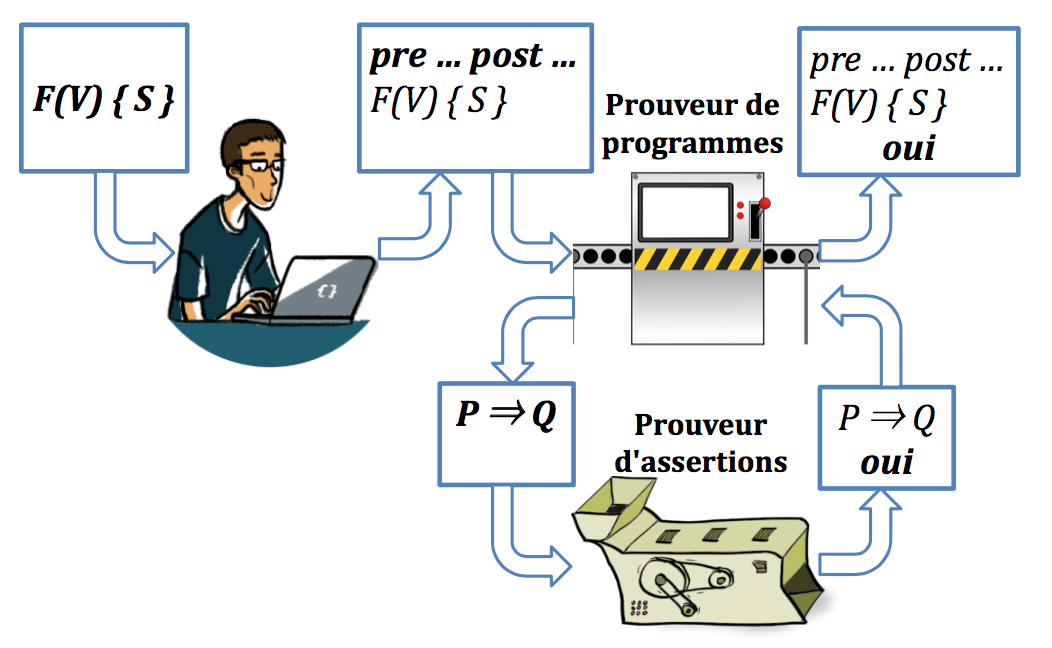
\includegraphics[width=\textwidth]{img/proof.png}
	\caption{Preuve automatique.}
\end{figure}

Le \textbf{programmeur} peut ajouter des assertions et
assomptions dans le programme.
Le \textbf{prouveur} peut ajouter des assertions
concernant les \textbf{erreurs d'exécution}.
Le prouveur de programme prouve
\begin{itemize}
	\item la \textbf{correction partielle} sur toutes les procédures et
	\item la \textbf{décroissance des variants} spécifiés.
\end{itemize}
Si des variants sont spécifiés sur toutes les boucles et procédures récursives,
alors on prouve la \textbf{correction totale}.

Le prouveur d'assertions reçoit en entrée une assertion $P[V]$
avec des variables $V$.
À la sortie, l'état est valide si $\forall V: P[V]$
ou invalide si $\exists V: \lnot P [V]$.

\subsubsection{Théories}
Les assertions comportent des \textbf{prédicats} et
des \textbf{fonctions} de signification définie.
Une \textbf{théorie} est l'ensemble des propriétés (assertions)
satisfaites par un ensemble d'opérations et de fonctions donné.

\subsubsection{Solveurs SMT}
Comme prouveur d'assertions,
on utilise des solveurs SMT (Satisfaisabilité Modulo Théories).
On ne sait pas répondre valide/invalide pour toute assertion $P$.
La logique du premier ordre est \textbf{indécidable},
il n'\textbf{existe pas} de procédure qui décide la validité pour tout $P$.
La validité est \textbf{semi-décidable}, on peut énumérer les $P$ valides.
Cela aussi dépend des \textbf{fonctions et prédicats} utilisés dans $P$
car un solveur ne supporte que certaines théories,
par exemple l'\textbf{arithmétique liéaire}.
Un solveur SMT peut répondre \og je ne sais pas\fg.

\subsection{Preuves de programme en Dafny}
Dafny est un langage de programmation orientée-objets avec spécifications.
En Dafny, pour vérifier les instructions, on inclut des \inlinedafny|assert|,
\inlinedafny|assume| et invariants de boucle.
Pour les méthodes, on utilise les pré/post, effets et variants.

\subsubsection{Expressions}
Les expressions de Dafny sont pures; il n'y a pas d'effets de bord
(\texttt{new}, \texttt{i++}).
Une assertion est une expression booléenne.
On utilise les opérateurs booléens \texttt{==>, <==, <==>, <=!=>}
et les quantificateurs \inlinedafny|forall| et \inlinedafny|forall|.

Pour définir une précondition on utilise \inlinedafny|requires|
suivi par la condition alors que pour une postcondition
on utilise \inlinedafny|ensures|.

\subsubsection{Boucles}
Il n'existe pas de boucles \texttt{for} en Dafny,
on n'utilise que des \inlinedafny|while|.
Le variant est inféré automatiquement par Dafny, mais si on veut l'introduire,
on utilise \inlinedafny|decreases| suivi par l'expression du variant.
Pour introduire l'invariant, on utilise \inlinedafny|invariant|.

Ensuite, si le paramètre $a$, par exemple un tableau, est modifié,
on écrit \inlinedafny|modifies a| après les pré/post de la méthode.

\subsubsection{Fonctions, prédicats et méthodes}
Les fonctions et les prédicats
(\inlinedafny|function|, \inlinedafny|predicate|)
peuvent uniquement être utilisés dans les spécifications.
\inlinedafny|function method| est utilisable
dans les spécifications et dans le code.
On ajoute \inlinedafny|reads| quand il faut lire les éléments du tableau
ou encore les champs d'un objet dans la fonction/prédicat.

\subsubsection{Structures de données}
Les invariants de représentation
(\inlinedafny|predicate ok() reads this {...}|)
sont à inclure dans la post des constructeurs et dans la pré/post des méthodes.
Les fonctions d'abstraction (\inlinedafny|function abs() reads this {...}|)
sont  à inclure dans la post des constructeurs est dans la post des méthodes.

Pour les assertions et les assomptions,
on utilise respectivement \inlinedafny|assert| et \inlinedafny|assume|.

\subsubsection{Types de données}
Les types de données en Dafny sont des \textbf{types-valeurs}:
ils n'ont pas de référence, sont immuables et ne sont jamais \inlinedafny|null|.
On les utilise comme domaines abstraits.
On a
\begin{itemize}
	\item les \textbf{séquences}: \inlinedafny|var l: seq<int> := [1,2,3];|;
	\item les \textbf{ensembles}: \inlinedafny|var s: set<int> := {1,2,3};|;
	\item les \textbf{multiensembles}:
	\inlinedafny|var b: multiset<int> := multiset{1,2,2,3,3};|;
	\item les \textbf{dictionnaires}:
	\inlinedafny|var m: map<int,bool> := map[1 := true, 2 := false];|.
\end{itemize}

\subsubsection{Variables et méthodes fantômes}
Les variables et méthodes fantômes, qui sont ignorées à l'exécution
mais sont prises en compte pour la vérification,
sont écrites de manière suivante en Dafny:
\inlinedafny|ghost var V:T;| et \inlinedafny|ghost method M(...):{}|.
Les fonctions et prédicats sont déjà fantômes.

L'expression \inlinedafny|ensures fresh(data)| dit qu'à la sortie,
\inlinedafny|data| est une \textbf{référence vers un objet frais}:
un objet nouvellement créé.
On peut toujours modifier un objet frais.
Par exemple, on l'utilise quand on redimensionne
un tableau au sein d'une méthode.

\subsubsection{Aliasing}
\begin{mydef}[Aliasing]
	L'\emph{aliasing} arrive lorsqu'on a une référence partagée.
\end{mydef}
Il faut toujours spécifier qu'il n'y a pas d'aliasing,
car les invariants ne peuvent pas être prouvés sinon.

\section{Programmation orientée-objets}
\subsection{Concepts}
Les caractèrisques majeurs de la POO sont
\begin{itemize}
	\item l'\textbf{encapsulation}: objets = données + opérations
	(variables + méthodes);
	\item l'\textbf{héritage}: construction incrémentale, sous-typage et
	\item le \textbf{polymorphisme}:
	on peut avoir des réponses différentes pour la même requête.
\end{itemize}

\subsubsection{Objets}
\begin{mydef}
	Un \emph{objet} est un composant de l'exécution,
	identifiable par référence.
	Les \emph{attributs} sont les données de l'objet,
	alors que les \emph{méthodes} sont ses opérations.
	Les \emph{constructeurs} sont des opérations qui créent un nouvel objet.
\end{mydef}

\subsubsection{Classes et interfaces}
\begin{mydef}
	Une \emph{classe} est un module logiciel définissant des objets.
	Une \emph{interface} est un ensemble
	d'attributs et d'opérations visibles.
	Une \emph{classe abstraite} (\inlinedafny|Traits| en Dafny)
	est une classe avec certaines méthodes non implémentées.
	Une interface est type abstrait de classe.
\end{mydef}

\subsubsection{Héritage}
\begin{mydef}[Héritage]
	L'\emph{héritage} consiste à définir une nouvelle classe ou interface
	en réutilisant et étendant une classe ou interface existante.
\end{mydef}

\subsubsection{Sous-typage}
\begin{mydef}[Sous-type]
	$A$ est un \emph{sous-type} de $B$ si et seulement si
	\begin{itemize}
		\item tous les objets de type $A$ sont de type $B$ et
		\item les fonctionnalités de $A$ \textbf{incluent}
		les fonctionnalités de $B$.
	\end{itemize}
	Si $A$ étend ou implémente $B$,
	alors $A$ est un \emph{sous-type} de $B$.
\end{mydef}

\subsubsection{Liaison et polymorphisme}
\begin{mydef}
	Soit une variable $v:T$ qui réfère à un objet $o:C$
	où $C$ (avec méthodes $m()$ et $n()$)
	est un sous-type de $T$ (avec méthode $m()$).
	\begin{itemize}
		\item Le \emph{typage statique} dit que
		seules les méthodes de $T$ peuvent être invoquées sur $v$.
		\item La \emph{liaison dynamique} dit que
		quand on invoque une méthode $v.m()$,
		c'est $C.m()$ qui est exécutée.
		\item Le \emph{polymorphisme} dit qu'un même appel à $m()$
		peut exécuter différentes implémentations de $m()$.
	\end{itemize}
\end{mydef}

\subsubsection{Diagrammes de classe}
Pour indiquer que les attributs ou les méthodes sont privés ou publiques,
on met à côté d'eux un $-$ ou $+$, respectivement.
\begin{figure}[H]
	\centering
	\begin{subfigure}{.48\textwidth}
		\centering
		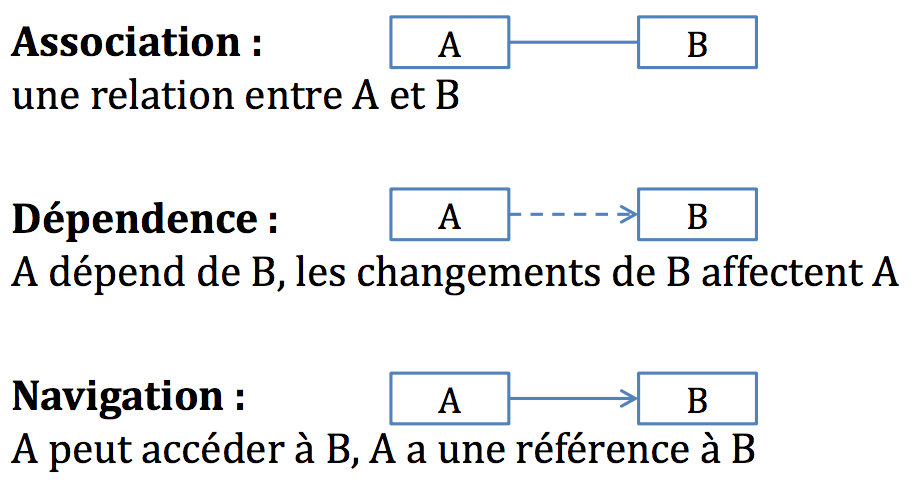
\includegraphics[width=\textwidth]{img/DC1.png}
	\end{subfigure}\hfill
	\begin{subfigure}{.48\textwidth}
		\centering
		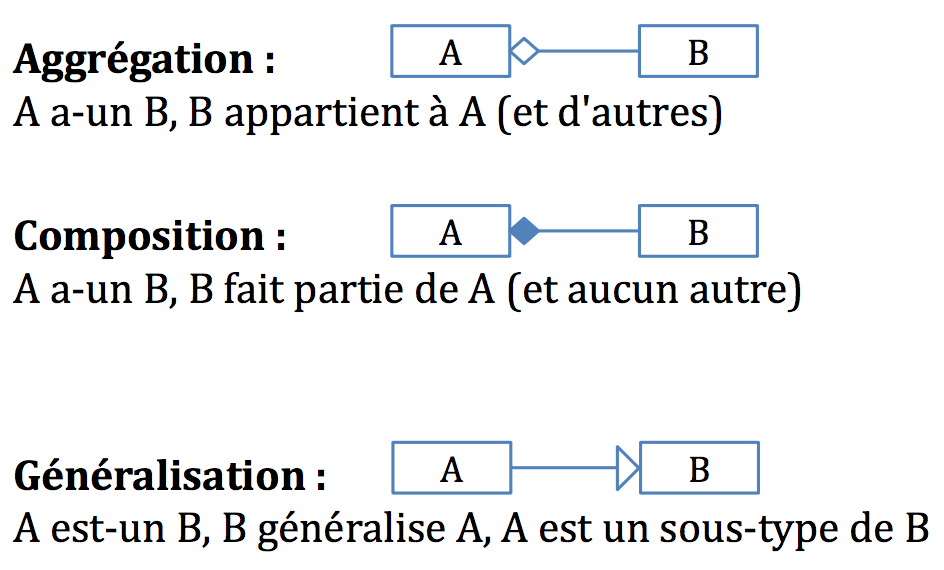
\includegraphics[width=\textwidth]{img/DC2.png}
	\end{subfigure}
	\caption{Diagrammes de classe: relations.}
\end{figure}

\paragraph{Multiplicités}
\begin{figure}[H]
	\centering
	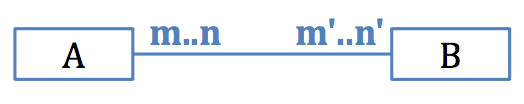
\includegraphics[width=0.4\textwidth]{img/multi.png}
\end{figure}
Chaque $A$ est associé avec entre \(m'\) et \(n'\) $B$,
alors que chaque \(B\) est associé avec entre \(m\) et \(n\) \(A\).
Quelques cas spéciaux:
\begin{itemize}
	\item $n$ ou $n..n$: exactement $n$;
	\item $*$ ou $0..*$: n'importe combien;
	\item $0..1$: zéro ou un;
	\item $1..*$: au moins un.
\end{itemize}
Par défaut la valeur est indéfinie.

\subsection{Héritage vs composition}
\begin{figure}[H]
	\centering
	\begin{subfigure}{.48\textwidth}
		\centering
		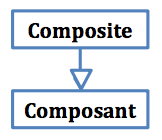
\includegraphics[width=\textwidth]{img/herit.png}
	\end{subfigure}\hfill
	\begin{subfigure}{.48\textwidth}
		\centering
		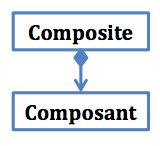
\includegraphics[width=\textwidth]{img/compo.png}
	\end{subfigure}
	\caption{Héritage vs composition.}
\end{figure}
\begin{table}[H]
	\centering
	\begin{tabular}{ll}
	\toprule
	Héritage & Composition \\
	\midrule
	Méthodes de Composant invocables directement &
	Méthodes de Composant doivent être redirigées \\
	Composite sous-type de Composant & Composite non lié à Composant \\
	Composant visible sur Composite & Composant pas visible sur Composite \\
	Instance de Composant fixée par construction &
	Instance de Composant peut varier à l'exécution \\
	Un seul Composant & Plusieurs composants de types variés \\
	Composant est une classe & Composant peut être une interface \\
	\bottomrule
	\end{tabular}
\end{table}

On préfère en général la composition à l'héritage;
on n'utilise l'héritage que dans le cas où le sous-typage est utile.

\subsection{Substitutivité}
\begin{mylaw}[Principe de substitutivité -- Loi de Liskov]
	Un sous-type doit \textbf{respecter le contrat} de son super-type,
	de sorte qu'une instance du sous-type
	soit \textbf{substituable} à une instance du super-type.
\end{mylaw}

\begin{mydef}[Substitutivité]
Soit deux méthodes
\(\texttt{U}_{\texttt{super}}\ \texttt{Super.m(T}_{\texttt{super}} \texttt{x)}\)
et \(\texttt{U}_{\texttt{sub}}\ \texttt{Sub.m(T}_{\texttt{sub}} \texttt{x)}\).
\texttt{Sub.m()} est \emph{substituable} pour \texttt{Super.m()}
si \texttt{Sub.m()} accepte des paramètres de type \(\texttt{T}_\texttt{super}\)
et retourne un résultat de type \(\texttt{U}_\texttt{super}\).
On a donc que \(\texttt{T}_\texttt{super}\) est
un sous-type de \(\texttt{T}_\texttt{sub}\)
et que \(\texttt{U}_\texttt{sub}\) est
un sous-type de \(\texttt{U}_\texttt{super}\).
\end{mydef}

Les spécifications de \texttt{Sub.m()} doivent respecter
les spécifications de \texttt{Super.m()}.
\begin{itemize}
	\item Pour la précondition,
	\(P_\texttt{super} \implies P_\texttt{sub}\).
	\item Pour la postcondition,
	\(P_\texttt{super} \implies (Q_\texttt{sub} \implies Q_{\texttt{super}})\).
\end{itemize}
Dans ce cas, $[P_\texttt{sub}]\ \texttt{Sub.m()}\ [Q_{\texttt{sub}}] \implies [P_{\texttt{super}}]\ \texttt{Super.m()}\ [Q_{\texttt{super}}]$.

\begin{figure}[H]
	\centering
	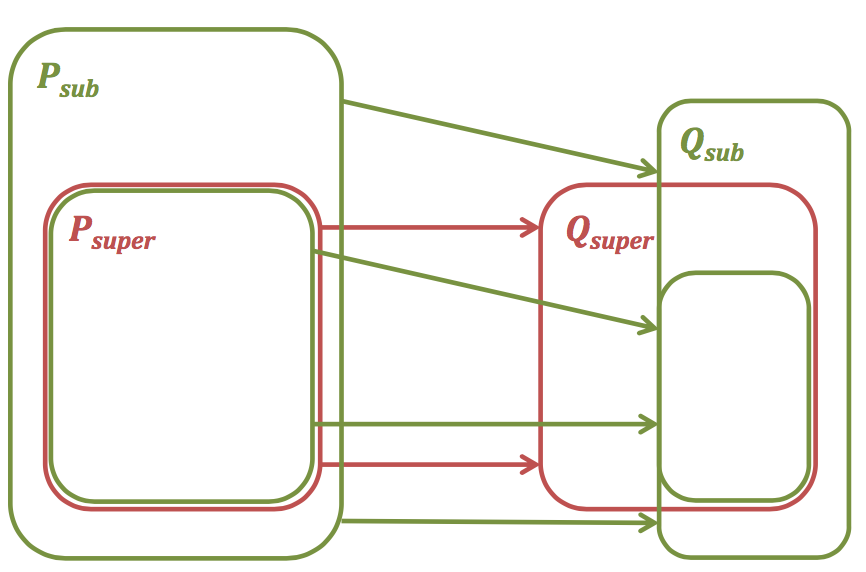
\includegraphics[width=0.7\textwidth]{img/subst.png}
\end{figure}


\subsection{Modularité, couplage et cohésion}
\begin{mydef}[Modularité]
	Un programme OO est \emph{modulaire}
	si des \textbf{problèmes différents} sont traités
	dans des \textbf{modules différents}.
	Pour maximiser la \textbf{cohésion}
	on ajoute l'interdépendence au sein d'un module.
	Pour minimiser le \textbf{couplage},
	on ajoute l'interdépendance entre les modules.
\end{mydef}

\begin{mylaw}[Principe de moindre connaissance]
	Un module ne doit avoir connaissance que des modules
	qui lui sont directement relatifs.
\end{mylaw}

\section{Patrons de conception}
\begin{mydef}[Patron de conception]
	Un \emph{patron de conception} (\emph{design pattern})
	est un \textbf{arrangement} caractéristique de \textbf{modules},
	permettant de résoudre un \textbf{problème de conception}
	en suivant certains \textbf{principes de conception}.
\end{mydef}

\begin{mydef}[Patron d'architecture]
	Un \emph{patron d'architecture}
	est une solution générale pour l'organisation d'ensemble d'un logiciel.
\end{mydef}

\subsection{Éléments d'un patron}
Les éléments d'un patron sont
\begin{itemize}
	\item le \textbf{nom}, pour faciliter la référence;
	\item le \textbf{problème}:
	\og quand peut-on l'appliquer et pour quels objectifs\fg;
	\item la \textbf{solution}: les éléments
	(classes, interfaces, variables, méthodes) et les relations entre eux;
	\item les \textbf{conséquences}: bénéfices, possibilités,
	coûts, compromis.
\end{itemize}

\subsection{Patrons GOF}
\subsubsection{Le patron \texttt{Factory Method}}
\paragraph{Problème}
Créer des objets d'un type donné sans fixer leur classe concrète.

\paragraph{Solution}
Une \textbf{méthode fabrique}.
On peut avoir plusieurs méthodes fabriques différentes.
On peut aussi grouper des méthodes fabriques dans une \textbf{classe fabrique}.

\begin{figure}[!htbp]
	\centering
	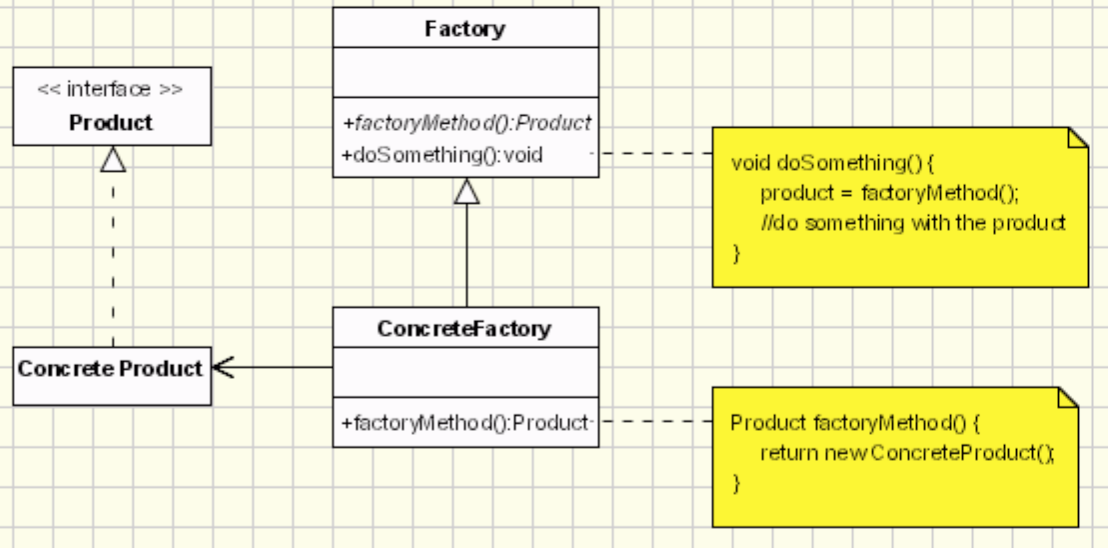
\includegraphics[width=0.7\textwidth]{img/factorymethod}
	\caption{Diagramme de classes du patron \texttt{Factory Method}.}
\end{figure}

\subsubsection{Le patron \texttt{Abstract Factory}}
\paragraph{Problème}
Créer des familles d'objets dépendants sans fixer leur classe concrète.

\paragraph{Solution}
Une interface qui définit des méthodes fabriques pour chaque type d'objet.
Pour chaque famille, une instance de cette interface
dont les méthodes gènérent les objets de la famille.
Cela permet de \textbf{réduire fortement la dépendance}
sur les différentes familles:
seul le module qui crée l'objet fabrique dépend des familles.
L'objet fabrique doit être \textbf{transmis à tous les modules}
qui créent des objets de la famille.

\begin{figure}[!htbp]
	\centering
	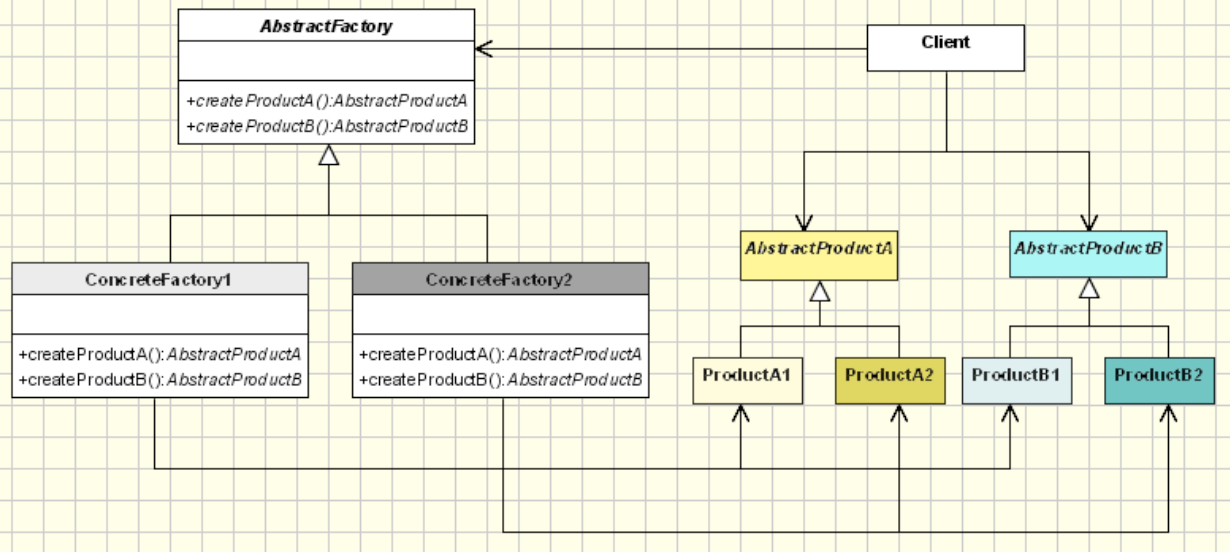
\includegraphics[width=0.7\textwidth]{img/abstractfactory}
	\caption{Diagramme de classes du patron \texttt{Abstract Factory}.}
\end{figure}

\subsubsection{La patron \texttt{FlyWeight}}
\paragraph{Problème}
Supporter une très grand nombre d'objets identiques.

\paragraph{Solution}
\textbf{Partager un seul objet} pour toutes les instances identiques.
Ce patron utilise une \textbf{méthode fabrique}
pour générer les instances.
Il distingue aussi l'état \textbf{intrinsèque}
(immutable, invariable, stocké dans l'objet) et
l'état \textbf{extrinsèque}
(mutable, variable, passé en paramètre aux méthodes).
Les objets gérés doivent être immutables.

\begin{figure}[!htbp]
	\centering
	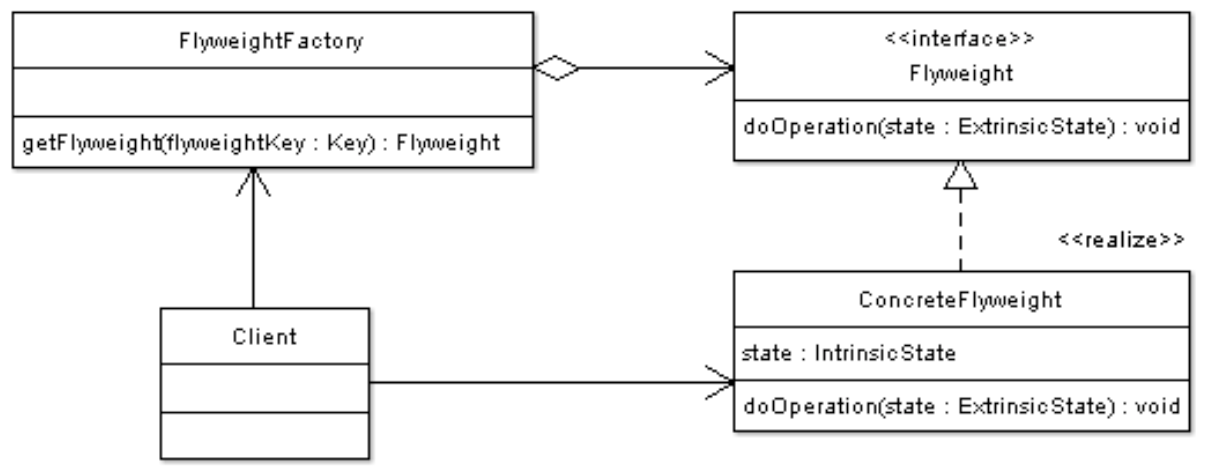
\includegraphics[width=0.7\textwidth]{img/flyweight}
	\caption{Diagramme de classes du patron \texttt{FlyWeight}.}
\end{figure}

\subsubsection{Le patron \texttt{Singleton}}
\paragraph{Problème}
Une classe avec une seule instance, globalement accessible.

\paragraph{Solution}
Créer et donne accès à \textbf{une instance} et
empêcher la création d'autres instances (constructeur privé).

\begin{figure}[!htbp]
	\centering
	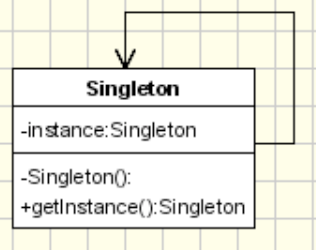
\includegraphics[width=0.7\textwidth]{img/singleton}
	\caption{Diagramme de classes du patron \texttt{Singleton}.}
\end{figure}

\subsubsection{Le patron \texttt{Filter}}
\paragraph{Problème}
Définir des \textbf{objets} qui représentent des \textbf{procédures}.

\paragraph{Solution}
Des \textbf{objets} qui contiennent une procédure comme \textbf{méthode}.

\begin{mydef}[Fermeture]
	Une \emph{fermeture} (\textit{closure})
	est une procédure dont certaines variables sont déjà liées.
\end{mydef}

\begin{figure}[!htbp]
	\centering
	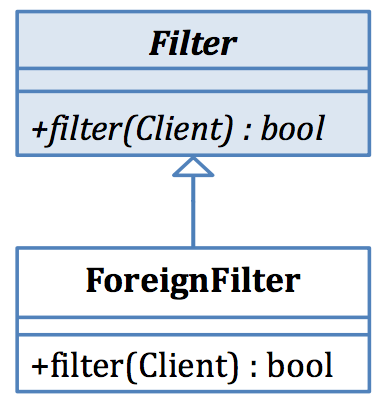
\includegraphics[width=0.7\textwidth]{img/filter}
	\caption{Diagramme de classes du patron \texttt{Filter}.}
\end{figure}

\subsubsection{Le patron \texttt{Strategy}}
\paragraph{Problème}
Définir une famille de procédures encapsulées et interchangeables
pour une fonctionnalité donnée.

\paragraph{Solution}
Une interface avec une méthode correspondant à la procédure.

\begin{figure}[!htbp]
	\centering
	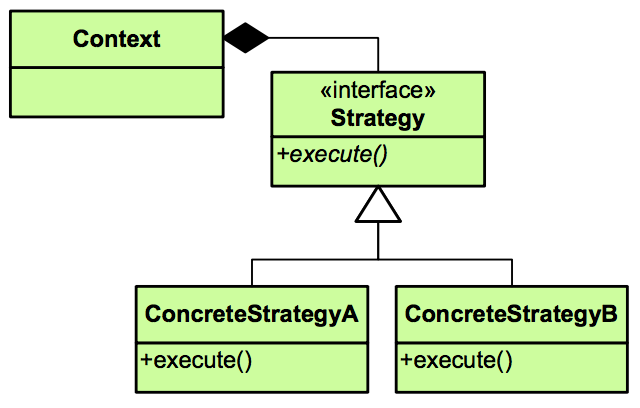
\includegraphics[width=0.7\textwidth]{img/strategy}
	\caption{Diagramme de classes du patron \texttt{Strategy}.}
\end{figure}

\paragraph{Discussion}
\begin{itemize}
	\item La stratégie n'a \textbf{pas d'effets}.
	\item Les \textbf{données} du contexte
	sont fournies en \textbf{paramètre} de la stratégie
	et/ou à la \textbf{construction} de la stratégie.
	\item \textbf{Modulaire}, \textbf{extensible} et
	évite des conditionnelles.
\end{itemize}

\subsubsection{Le patron \texttt{Command}}
\paragraph{Problème}
Définir une famille de requêtes encapsulées et interchangeables
pour des comportements quelconques.

\paragraph{Solution}
Une interface avec une méthode correspondant à la requête.

\begin{figure}[!htbp]
	\centering
	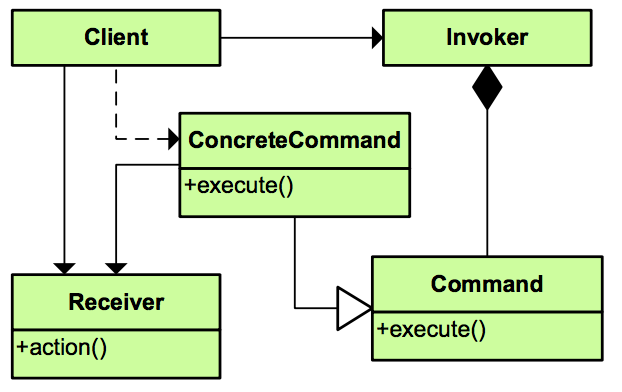
\includegraphics[width=0.7\textwidth]{img/command}
	\caption{Diagramme de classes du patron \texttt{Command}.}
\end{figure}

\paragraph{Discussion}
\begin{itemize}
	\item La commande n'a \textbf{pas de résultat}
	mais produit \textbf{un effet}.
	\item Les \textbf{données} du contexte sont fournies
	à la \textbf{construction} de la commande.
	\item \textbf{Modulaire}, \textbf{extensible} et
	évite des conditionnelles.
	\item Les commandes peuvent être \textbf{postposées},
	mises en \textbf{files}, \textbf{transférées},
	\textbf{rejouées}, \ldots
	\item Supporte \texttt{undo} avec une méthode supplémentaire.
\end{itemize}

\subsubsection{Le patron \texttt{Observer}}
\paragraph{Problème}
Définir un lien entre objets tel que quand un objet est modifié,
ses dépendants sont notifiés.

\paragraph{Solution}
\texttt{Subject.notify()} invoque \texttt{o.update()}
pour tous les observateurs \texttt{o} attachés.

\paragraph{Notification}
\begin{table}[H]
	\centering
	\begin{tabular}{lll}
		& Push & Pull\\
		\toprule
		Accès à la source & Fournie en paramètre de \texttt{update()} & Observateur doit y accéder par d'autres moyens\\
		\midrule
		Données & \textbf{Plus de données} que nécessaire & Accède uniquement aux \textbf{données nécessaires}\\
		\bottomrule
	\end{tabular}
	\caption{Comparaison entre la construction push et pull.}
\end{table}

\begin{figure}[!htbp]
	\centering
	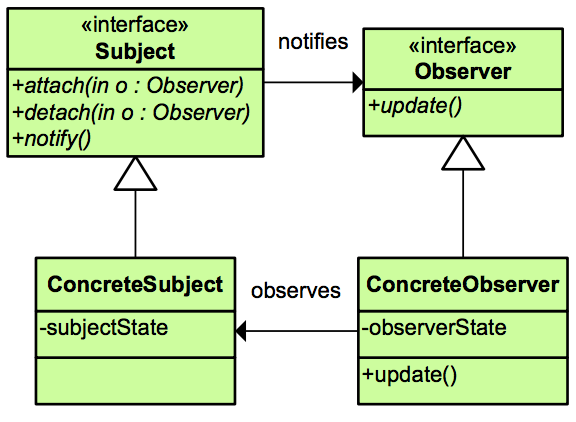
\includegraphics[width=0.7\textwidth]{img/observer}
	\caption{Diagramme de classes du patron \texttt{Observer}.}
\end{figure}

\paragraph{Discussion}
\begin{itemize}
	\item Aussi appelé \texttt{Publish-Subscribe} ou \texttt{Dependents}.
	\item \textbf{Faible couplage}:
	le sujet dépend uniquement de l'\textbf{interface} \texttt{Observer}.
	\item \textbf{Un sujet} peut être observé
	par \textbf{plusieurs observateurs}.
	\item \textbf{Un observateur} peut observer \textbf{plusieurs sujets}.
\end{itemize}

\subsubsection{Le patron \texttt{Composite}}
\paragraph{Problème}
Définir une structure hiérarchique de contenants et contenus,
en traitant uniformément les éléments individuels et composés.

\paragraph{Solution}
\texttt{Composite} \textbf{hérite} et est \textbf{composée}
de \texttt{Component}.

\begin{figure}[!htbp]
	\centering
	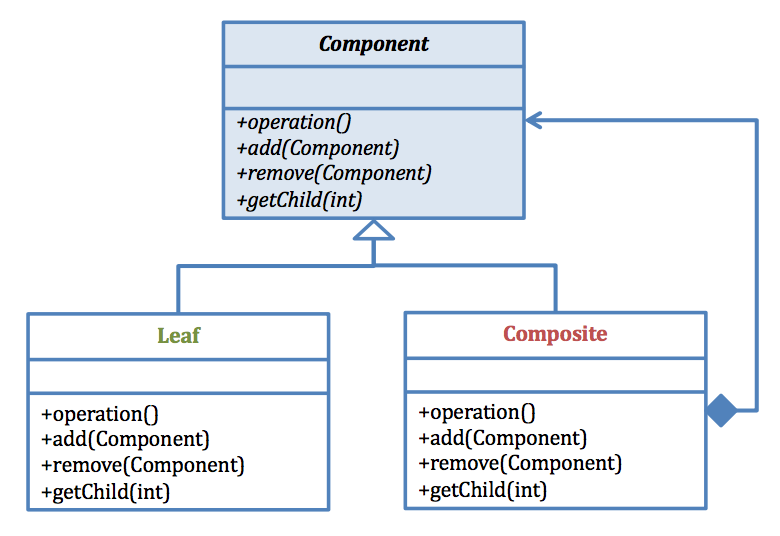
\includegraphics[width=0.7\textwidth]{img/composite}
	\caption{Diagramme de classes du patron \texttt{Composite}.}
\end{figure}

\paragraph{Discussion}
\begin{itemize}
	\item Simplifie les clients:
	composants primitifs et conteneurs traités uniformément.
	\item On peut facilement ajouter des types de composants nouveaux.
	\item Maximiser les opérations offertes sur \texttt{Component}.
	\begin{itemize}
		\item \texttt{Component} donne une implémentation par défaut,
		les sous-classes les redéfinissent.
		\item Parfois trop général,
		opérations non définies pour certains types de composants.
	\end{itemize}
\end{itemize}

\subsubsection{Le patron \texttt{Interpreter}}
\paragraph{Problème}
Définir un calcul sur une structure arborescente
(représentant les phrases d'un langage).

Par exemple, le problème du double dispatch
possède deux solutions sub-optimales:
\begin{itemize}
	\item Une classe par calcul.
	\begin{itemize}
		\item \textbf{Facile} d'ajouter un \textbf{nouveau calcul}.
		\item \textbf{Difficile} d'ajouter
		un \textbf{type d'expression}.
		\item On peut décomposer
		en sous-méthodes par type d'expression.
		\item On pourrait avoir une \textbf{interface abstraite},
		avec le patron \texttt{Strategy}.
	\end{itemize}
	\item Une classe par expression.
	\begin{itemize}
		\item \textbf{Facile} d'ajouter un \textbf{type d'expression}.
		\item \textbf{Difficile} d'ajouter un \textbf{calcul}.
	\end{itemize}
\end{itemize}

\paragraph{Solution}
Une méthode \texttt{interpret} sur toutes les classes de l'arborescence.

\begin{figure}[!htbp]
	\centering
	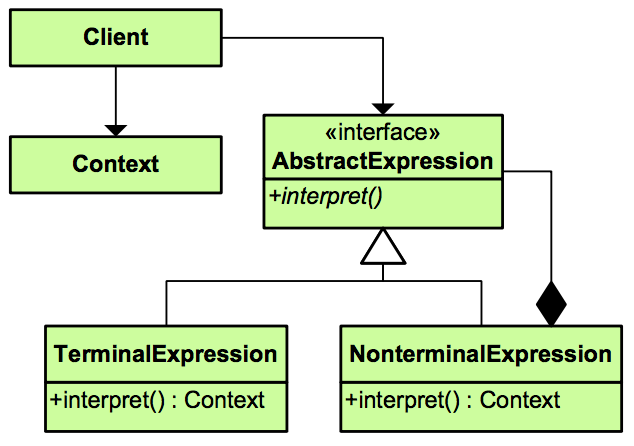
\includegraphics[width=0.7\textwidth]{img/interpreter}
	\caption{Diagramme de classes du patron \texttt{Interpreter}.}
\end{figure}

\paragraph{Discussion}
\begin{itemize}
	\item Basé sur le patron \texttt{Composite}.
	\item Défini pour \textbf{interpréter un langage},
	mais applicable à tout \textbf{autre type de structure composée}.
	\item Extension du langage facile.
	\item Ajout de fonctions d'interprétation difficile.
\end{itemize}

\subsubsection{Le patron \texttt{Visitor}}
\paragraph{Problème}
Définir plusieurs calculs sur une structure,
sans changer les classes de la structure.

\paragraph{Solution}
\texttt{ElementA.accept(v)} appelle \texttt{visitElementA(this)}.

\begin{figure}[!htbp]
	\centering
	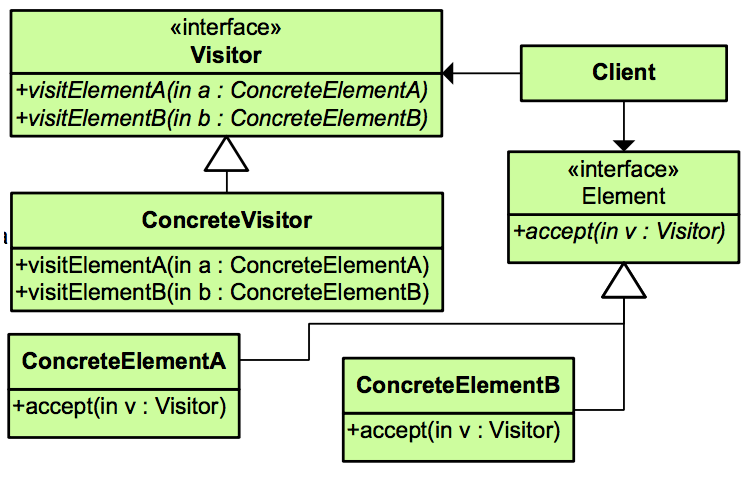
\includegraphics[width=0.7\textwidth]{img/visitor}
	\caption{Diagramme de classes du patron \texttt{Visitor}.}
\end{figure}

\paragraph{Discussion}
\begin{itemize}
	\item \textbf{Modulaire}, groupe un calcul dans une classe.
	\item Peut s'appliquer à \textbf{toute structure},
	pas uniquement les \texttt{Composite}.
	\item Réalise un \textbf{double dispatch}:
	\texttt{accept} dispatche sur le type d'expression,
	\texttt{visitElement} dispatche sur le calcul.
	\item Les visités doivent pouvoir \textbf{fournir les informations}
	nécessaires au calcul.
	\item On peut mettre le \textbf{parcours} de la structure
	\textbf{dans le visiteur}.
	Il est donc plus précis, en fonction du calcul,
	mais répété pour chaque visiteur.
\end{itemize}
\end{document}
